% =============================================================================
%  Diplomado en Data Science Aplicada con Python para la Toma de Decisiones
%  Clase 17: Árboles de Decisión --- El Modelo que se Explica Solo
%  Arca Continental Ecuador | UDLA
%
%  Compilar: pdflatex -shell-escape presentacion.tex (x2 para refs)
% =============================================================================
\documentclass[aspectratio=169, 11pt]{beamer}

\usepackage[T1]{fontenc}
\usepackage[utf8]{inputenc}
\usepackage[spanish,es-noshorthands]{babel}
\usepackage{FiraSans}
\usepackage{FiraMono}
\renewcommand{\familydefault}{\sfdefault}
\usepackage{graphicx}
\usepackage{tikz}
\usetikzlibrary{arrows.meta, positioning, shapes.geometric, shapes.misc,
  calc, fit, decorations.pathreplacing, backgrounds}
\usepackage{fontawesome5}
\usepackage{minted}
\usepackage{tcolorbox}
\tcbuselibrary{minted, skins, breakable}
\usepackage{booktabs}
\usepackage{colortbl}
\usepackage{multicol}
\usepackage{hyperref}
\usepackage{calc}
\usepackage{amsmath}

\definecolor{arcaRed}{HTML}{C82B40}
\definecolor{arcaDark}{HTML}{6B1525}
\definecolor{udlaCrimson}{HTML}{A31545}
\definecolor{arcaGray}{HTML}{F5F5F5}
\definecolor{arcaLightGray}{HTML}{EBEBEB}
\definecolor{textDark}{HTML}{2D2D2D}
\definecolor{textMuted}{HTML}{6B7280}
\definecolor{codeGreen}{HTML}{16A34A}
\definecolor{codeBlue}{HTML}{2563EB}
\definecolor{codeOrange}{HTML}{EA580C}
\definecolor{codePurple}{HTML}{7C3AED}

\usetheme{default}
\usecolortheme{default}
\setbeamertemplate{navigation symbols}{}
\setbeamertemplate{footline}{}
\setbeamertemplate{headline}{}
\setbeamercolor{normal text}{fg=textDark}
\setbeamercolor{frametitle}{fg=arcaRed, bg=white}
\setbeamercolor{title}{fg=white}
\setbeamercolor{subtitle}{fg=white!85}
\setbeamercolor{author}{fg=white!80}
\setbeamercolor{date}{fg=white!70}
\setbeamercolor{item}{fg=arcaRed}
\setbeamercolor{subitem}{fg=arcaDark}
\setbeamercolor{block title}{fg=white, bg=arcaRed}
\setbeamercolor{block body}{fg=textDark, bg=arcaGray}
\setbeamercolor{block title alerted}{fg=white, bg=codeOrange}
\setbeamercolor{block body alerted}{fg=textDark, bg=arcaGray}
\setbeamercolor{block title example}{fg=white, bg=codeGreen}
\setbeamercolor{block body example}{fg=textDark, bg=arcaGray}
\setbeamercolor{section in toc}{fg=arcaDark}
\setbeamerfont{frametitle}{size=\Large, series=\bfseries}
\setbeamerfont{title}{size=\huge, series=\bfseries}
\setbeamerfont{subtitle}{size=\large}
\setbeamerfont{author}{size=\normalsize}
\setbeamerfont{date}{size=\small}
\setbeamerfont{block title}{size=\normalsize, series=\bfseries}
\setbeamerfont{footnote}{size=\tiny}
\setbeamertemplate{itemize item}{\scriptsize\raise1.5pt\hbox{\color{arcaRed}$\blacktriangleright$}}
\setbeamertemplate{itemize subitem}{\scriptsize\raise1pt\hbox{\color{arcaDark}$\bullet$}}
\setbeamertemplate{enumerate items}[default]
\setbeamercolor{enumerate item}{fg=arcaRed}

\setbeamertemplate{headline}{%
  \begin{tikzpicture}[remember picture, overlay]
    \fill[arcaDark] (current page.north west) rectangle
      ([yshift=-0.7cm]current page.north east);
    \node[anchor=west, inner sep=0pt] at
      ([xshift=0.6cm, yshift=-0.35cm]current page.north west)
      {
\includegraphics[height=0.45cm]{../logo_udla_white.png}};
    \node[anchor=east, inner sep=0pt] at
      ([xshift=-0.6cm, yshift=-0.35cm]current page.north east)
      {
\includegraphics[height=0.45cm]{../ArcaContinental_white.png}};
  \end{tikzpicture}%
  \vspace{0.7cm}%
}

\setbeamertemplate{footline}{%
  \begin{tikzpicture}[remember picture, overlay]
    \node[anchor=south east, font=\scriptsize\bfseries\color{arcaRed}] at
      ([xshift=-0.5cm, yshift=0.15cm]current page.south east)
      {\insertframenumber};
  \end{tikzpicture}%
  \vspace{0.3cm}%
}

\setbeamertemplate{frametitle}{%
  \vspace{0.25cm}%
  \usebeamerfont{frametitle}\usebeamercolor[fg]{frametitle}\insertframetitle%
  \par\vspace{2pt}%
  \begin{tikzpicture}
    \fill[arcaRed] (0,0) rectangle (3cm, 1.5pt);
    \fill[arcaLightGray] (3cm,0) rectangle (\textwidth, 0.5pt);
  \end{tikzpicture}%
  \vspace{0.1cm}%
}

\newtcblisting{pyblock}[1][]{%
  listing engine=minted, minted language=python, minted style=friendly,
  minted options={fontsize=\small, linenos=false, breaklines=true, python3=true},
  colback=arcaGray, colframe=arcaRed, left=4pt, right=4pt, top=4pt, bottom=4pt,
  boxrule=0pt, leftrule=3pt, arc=2pt, listing only, #1}

\newtcblisting{outputblock}[1][]{%
  listing engine=minted, minted language=text, minted style=bw,
  minted options={fontsize=\small, breaklines=true},
  colback=white, colframe=arcaLightGray, left=4pt, right=4pt, top=4pt, bottom=4pt,
  boxrule=0.5pt, arc=2pt, listing only,
  title={\small\faTerminal\hspace{6pt}Output}, coltitle=textMuted,
  fonttitle=\small\ttfamily, colbacktitle=white, #1}

\newcommand{\sectionframe}[2]{%
  \begingroup
  \setbeamertemplate{headline}{}%
  \setbeamertemplate{footline}{}%
  \begin{frame}[plain, noframenumbering]
    \begin{tikzpicture}[remember picture, overlay]
      \fill[arcaRed] (current page.south west) rectangle (current page.north east);
      \node[anchor=center, text=white, font=\Huge\bfseries, text width=12cm,
            align=center] at ([yshift=0.5cm]current page.center) {#1};
      \node[anchor=center, text=white!80, font=\large, text width=10cm,
            align=center] at ([yshift=-0.8cm]current page.center) {#2};
    \end{tikzpicture}
  \end{frame}
  \endgroup
}

\title{Diplomado en Data Science Aplicada\\con Python para la Toma de Decisiones}
\subtitle{Clase 17: Árboles de Decisión --- El Modelo que se Explica Solo}
\author{Carlos Enrique Mosquera Trujillo}
\date{22 de Abril, 2026}

\begin{document}

% ── PORTADA ──────────────────────────────────────────────────────────────────
{
\setbeamertemplate{headline}{}
\setbeamertemplate{footline}{}
\begin{frame}[plain, noframenumbering]
  \begin{tikzpicture}[remember picture, overlay]
    \fill[arcaDark] (current page.south west) rectangle (current page.north east);
    \fill[arcaRed] ([yshift=-3.5cm]current page.north west) rectangle
      ([yshift=-4.2cm]current page.north east);
    \node[anchor=west, inner sep=0pt] at
      ([xshift=1cm, yshift=-1.5cm]current page.north west)
      {
\includegraphics[height=1cm]{../logo_udla_white.png}};
    \node[anchor=east, inner sep=0pt] at
      ([xshift=-1cm, yshift=-1.5cm]current page.north east)
      {
\includegraphics[height=1cm]{../ArcaContinental_white.png}};
  \end{tikzpicture}
  \vspace{2.5cm}
  \begin{center}
    {\usebeamerfont{title}\usebeamercolor[fg]{title}\inserttitle\par}
    \vspace{0.4cm}
    {\usebeamerfont{subtitle}\usebeamercolor[fg]{subtitle}\insertsubtitle\par}
    \vspace{0.6cm}
    {\usebeamerfont{author}\usebeamercolor[fg]{author}\insertauthor\par}
    \vspace{0.15cm}
    {\usebeamerfont{date}\usebeamercolor[fg]{date}\insertdate\par}
  \end{center}
\end{frame}
}

% ── MÓDULO 4 ─────────────────────────────────────────────────────────────────
{
\setbeamertemplate{headline}{}
\setbeamertemplate{footline}{}
\begin{frame}[plain, noframenumbering]
  \begin{tikzpicture}[remember picture, overlay]
    \fill[arcaDark] (current page.south west) rectangle (current page.north east);
    \node[anchor=center, text=white, font=\Large\bfseries, text width=12cm,
          align=center] at ([yshift=1cm]current page.center)
      {Módulo 4 --- clase 4};
    \node[anchor=center, text=white!90, font=\huge\bfseries, text width=12cm,
          align=center] at ([yshift=-0.3cm]current page.center)
      {Machine Learning Supervisado};
  \end{tikzpicture}
\end{frame}
}

% ── ROADMAP ─────────────────────────────────────────────────────────────────
\begin{frame}[shrink=22]{Hoja de Ruta de Hoy}
  \vspace{-4pt}
  \begin{center}
  \begin{tikzpicture}[
    node distance=0.35cm,
    roadstep/.style={rectangle, rounded corners=4pt, draw=arcaRed, fill=arcaRed!8,
                 minimum width=11cm, minimum height=0.65cm,
                 font=\footnotesize\bfseries\color{arcaDark}, align=left,
                 text width=10cm, inner sep=6pt},
    num/.style={circle, fill=arcaRed, text=white, font=\scriptsize\bfseries,
                minimum size=0.5cm, inner sep=0pt},
  ]
    \node[roadstep] (s0) {\hspace{0.8cm}Curva ROC y AUC --- más allá del umbral 0.5};
    \node[roadstep, below=of s0] (s1) {\hspace{0.8cm}Curva Precision-Recall --- la correcta para desbalanceados};
    \node[roadstep, below=of s1] (s2) {\hspace{0.8cm}Umbral óptimo con lógica de negocio};
    \node[roadstep, below=of s2] (s3) {\hspace{0.8cm}Árboles de decisión: intuición, Gini, frontera};
    \node[roadstep, below=of s3] (s4) {\hspace{0.8cm}DecisionTreeClassifier: entrenar, podar, visualizar};
    \node[roadstep, below=of s4] (s5) {\hspace{0.8cm}Feature importance y comparación árbol vs logística};
    \node[roadstep, below=of s5] (s6) {\hspace{0.8cm}Gradio: del notebook a la demo interactiva};

    \node[num] at ([xshift=0.45cm]s0.west) {1};
    \node[num] at ([xshift=0.45cm]s1.west) {2};
    \node[num] at ([xshift=0.45cm]s2.west) {3};
    \node[num] at ([xshift=0.45cm]s3.west) {4};
    \node[num] at ([xshift=0.45cm]s4.west) {5};
    \node[num] at ([xshift=0.45cm]s5.west) {6};
    \node[num] at ([xshift=0.45cm]s6.west) {7};
  \end{tikzpicture}
  \end{center}
\end{frame}

% =============================================================================
%  BLOQUE A: CURVA ROC (DETALLE COMPLETO — desde clase 16)
% =============================================================================
\sectionframe{Curva ROC y AUC}{Más allá del umbral 0.5}

\begin{frame}[shrink=22]{El Modelo No Devuelve Etiquetas, Devuelve Probabilidades}
  \vspace{-4pt}
  {\footnotesize\color{arcaDark}\bfseries
    Cuando la regresión logística ``predice'', realmente responde:
    \textit{``hay un 67\% de probabilidad de que este paciente sufra un ACV''}.}

  \vspace{6pt}
  \begin{center}
    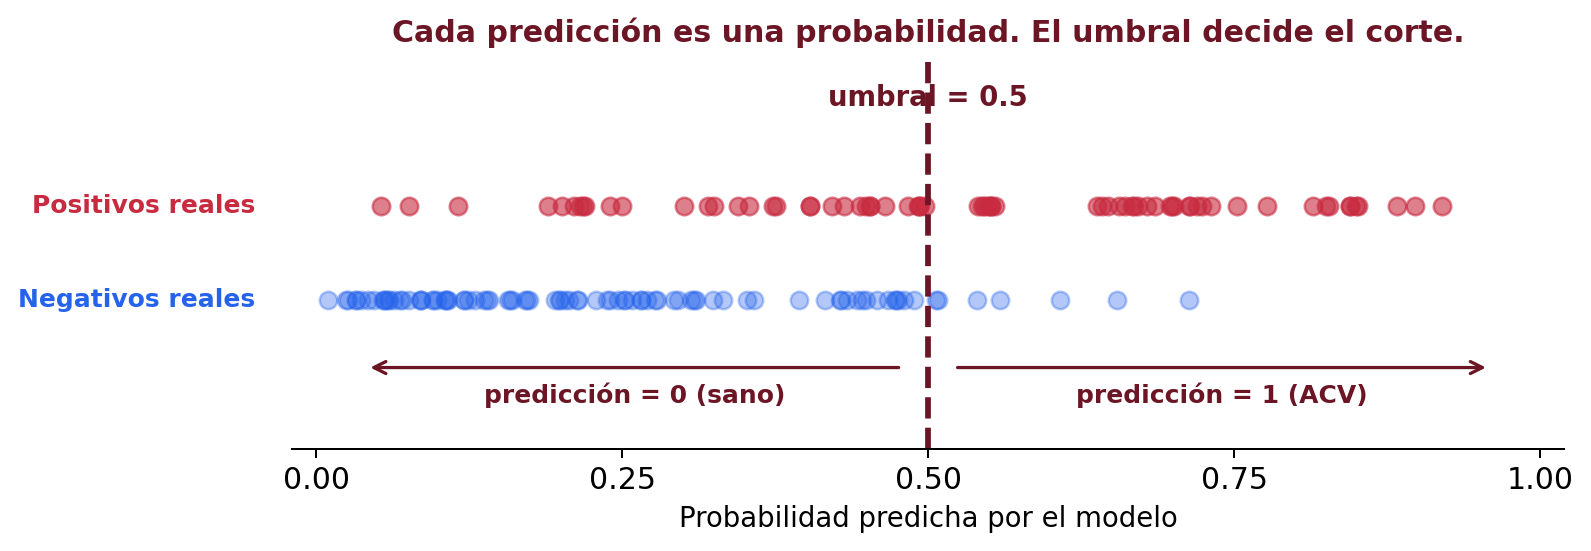
\includegraphics[width=0.85\textwidth]{fig_umbral.png}
  \end{center}

  \vspace{2pt}
  {\scriptsize\color{textMuted}
    Cada punto es un paciente. Rojo = tuvo ACV, azul = sano.
    La línea vertical es el \textbf{umbral}: todo lo que caiga a la derecha
    se clasifica como ``1'', a la izquierda como ``0''.}
\end{frame}

\begin{frame}[fragile,shrink=10]{\texttt{predict\_proba()} y el Umbral 0.5}
  \vspace{-4pt}
  {\footnotesize\color{arcaDark}\bfseries
    \texttt{predict()} usa por defecto un umbral de \textbf{0.5}.
    Pero 0.5 es una convención, no una ley.}

  \vspace{4pt}
  \begin{pyblock}
# Probabilidades reales del modelo
probs = modelo.predict_proba(X_test_s)[:, 1]
print(probs[:5])
# -> [0.08, 0.42, 0.67, 0.15, 0.91]

# Esto es lo que predict() hace internamente:
y_pred_default = (probs >= 0.5).astype(int)

# Pero podemos elegir OTRO umbral:
y_pred_sensible = (probs >= 0.3).astype(int)   # mas alertas
y_pred_estricto = (probs >= 0.7).astype(int)   # mas confianza
  \end{pyblock}

  \vspace{2pt}
  {\scriptsize\color{arcaDark}
    \faKey\hspace{4pt} El umbral es una \textbf{decisión de negocio}, no
    estadística. Lo elegimos según el costo del error.}
\end{frame}

\begin{frame}{La Curva ROC --- ¿Qué Mide?}
  \vspace{-4pt}
  {\footnotesize\color{arcaDark}\bfseries
    La curva \textbf{ROC} (Receiver Operating Characteristic) muestra cómo
    se comportan \texttt{TPR} y \texttt{FPR} para \textbf{cada umbral posible}.}

  \vspace{6pt}
  {\scriptsize
  \begin{tabular}{@{}lp{9cm}@{}}
    \toprule
    \textbf{TPR} (True Positive Rate) & \texttt{= VP / (VP + FN)} --- el \textbf{recall}. De los enfermos, ¿cuántos detecto? \\
    \textbf{FPR} (False Positive Rate) & \texttt{= FP / (FP + VN)} --- de los sanos, ¿a cuántos marqué mal como enfermos? \\
    \bottomrule
  \end{tabular}
  }

  \vspace{8pt}
  {\footnotesize
  \begin{itemize}\setlength{\itemsep}{4pt}
    \item[{\color{arcaRed}\scriptsize\faArrowRight}]
      \textbf{Umbral muy bajo} (0.01): detecto a todos (TPR=1) pero también
      marco sanos (FPR alto).
    \item[{\color{arcaRed}\scriptsize\faArrowRight}]
      \textbf{Umbral muy alto} (0.99): casi no marco a nadie (TPR=0, FPR=0).
    \item[{\color{arcaRed}\scriptsize\faArrowRight}]
      \textbf{La curva recorre todos esos puntos.}
  \end{itemize}
  }
\end{frame}

\begin{frame}{Cómo Se Calcula CADA Punto de la ROC}
  \vspace{-4pt}
  {\footnotesize\color{arcaDark}\bfseries
    Receta para \textbf{un} punto de la curva:}

  \vspace{4pt}
  {\footnotesize
  \begin{enumerate}\setlength{\itemsep}{3pt}
    \item Fijar un umbral $u$ (por ejemplo 0.20, 0.45, 0.70\ldots).
    \item Convertir probabilidades en predicciones: \texttt{y\_pred = (proba >= u)}.
    \item Contar VP, FN, FP, VN en la matriz de confusión.
    \item Calcular:
      $\text{TPR} = \dfrac{VP}{VP + FN}$, \quad
      $\text{FPR} = \dfrac{FP}{FP + VN}$
    \item Graficar el punto $(\text{FPR}, \text{TPR})$.
  \end{enumerate}
  }

  \vspace{4pt}
  \begin{tcolorbox}[colback=arcaRed!8, colframe=arcaRed, boxrule=0.5pt,
    arc=2pt, left=6pt, right=6pt, top=4pt, bottom=4pt]
    {\scriptsize\color{arcaDark}
    \faArrowRight\hspace{4pt}\textbf{Repetir} para \textbf{todos} los umbrales posibles
    (sklearn lo hace automáticamente, usando los scores únicos como umbrales).
    Los puntos conectados forman la curva.}
  \end{tcolorbox}
\end{frame}

\begin{frame}[shrink=42]{3 Umbrales = 3 Puntos en la Curva}
  \vspace{-4pt}
  \begin{center}
    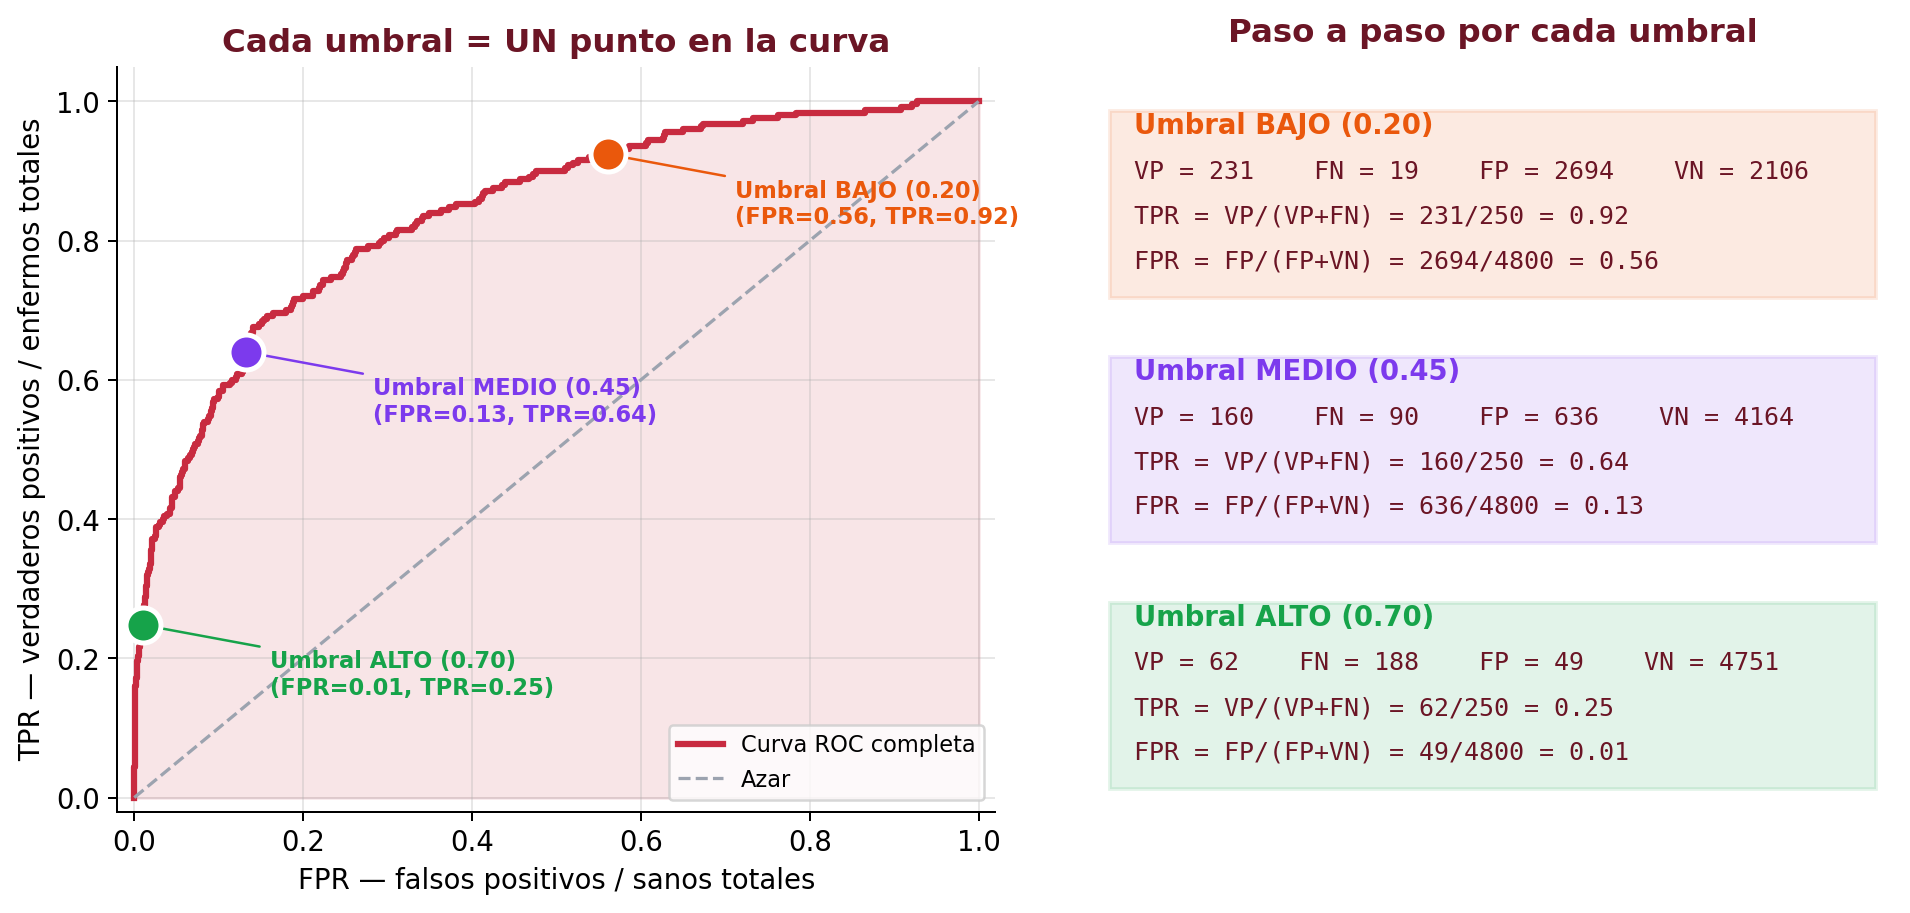
\includegraphics[width=0.82\textwidth]{fig_roc_puntos.png}
  \end{center}

  \vspace{-2pt}
  {\scriptsize\color{textMuted}
    \faLightbulb\hspace{4pt} Mismo modelo, mismos datos. Cambiando el
    umbral obtenemos puntos \textbf{distintos}. La curva es el lugar
    geométrico de TODOS los umbrales.}
\end{frame}

\begin{frame}[shrink=20]{¿Cómo Se Calcula el AUC?}
  \vspace{-4pt}
  {\footnotesize\color{arcaDark}\bfseries
    AUC = \textbf{Área Bajo la Curva}. No es ``sumar y dividir''
    --- es una integral numérica.}

  \vspace{6pt}
  \begin{columns}[T]
    \begin{column}{0.58\textwidth}
      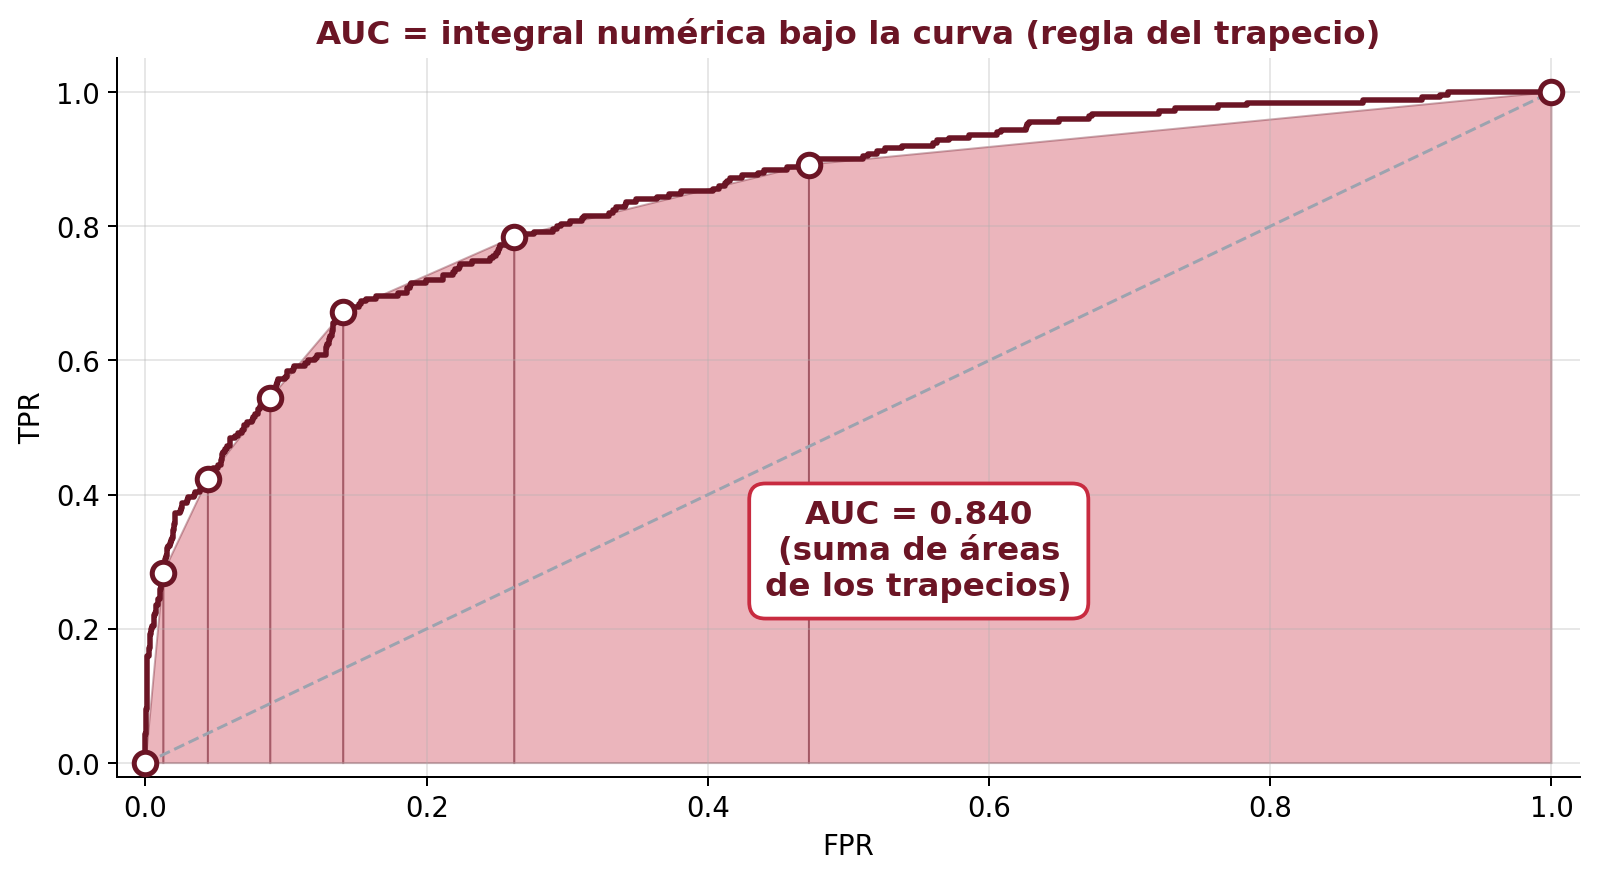
\includegraphics[width=\textwidth]{fig_auc_trapecios.png}
    \end{column}
    \begin{column}{0.40\textwidth}
      {\scriptsize\color{arcaDark}
      \textbf{Regla del trapecio:}
      \vspace{4pt}

      Entre dos puntos consecutivos $(x_i, y_i)$ y $(x_{i+1}, y_{i+1})$:
      $$\text{área}_i = (x_{i+1} - x_i) \cdot \frac{y_i + y_{i+1}}{2}$$

      \vspace{4pt}
      AUC total:
      $$\text{AUC} = \sum_i \text{área}_i$$

      \vspace{4pt}
      \texttt{sklearn.metrics.auc} hace exactamente esto.}
    \end{column}
  \end{columns}

  \vspace{4pt}
  {\scriptsize\color{textMuted}
    \faArrowRight\hspace{4pt} \textbf{Interpretación probabilística:} el AUC
    es la probabilidad de que el modelo dé un score más alto a un enfermo
    aleatorio que a un sano aleatorio. AUC = 0.84 → 84\% de las veces
    acierta el orden.}
\end{frame}

\begin{frame}[shrink=26]{Cómo Se Lee la Curva ROC}
  \vspace{-4pt}
  \begin{center}
    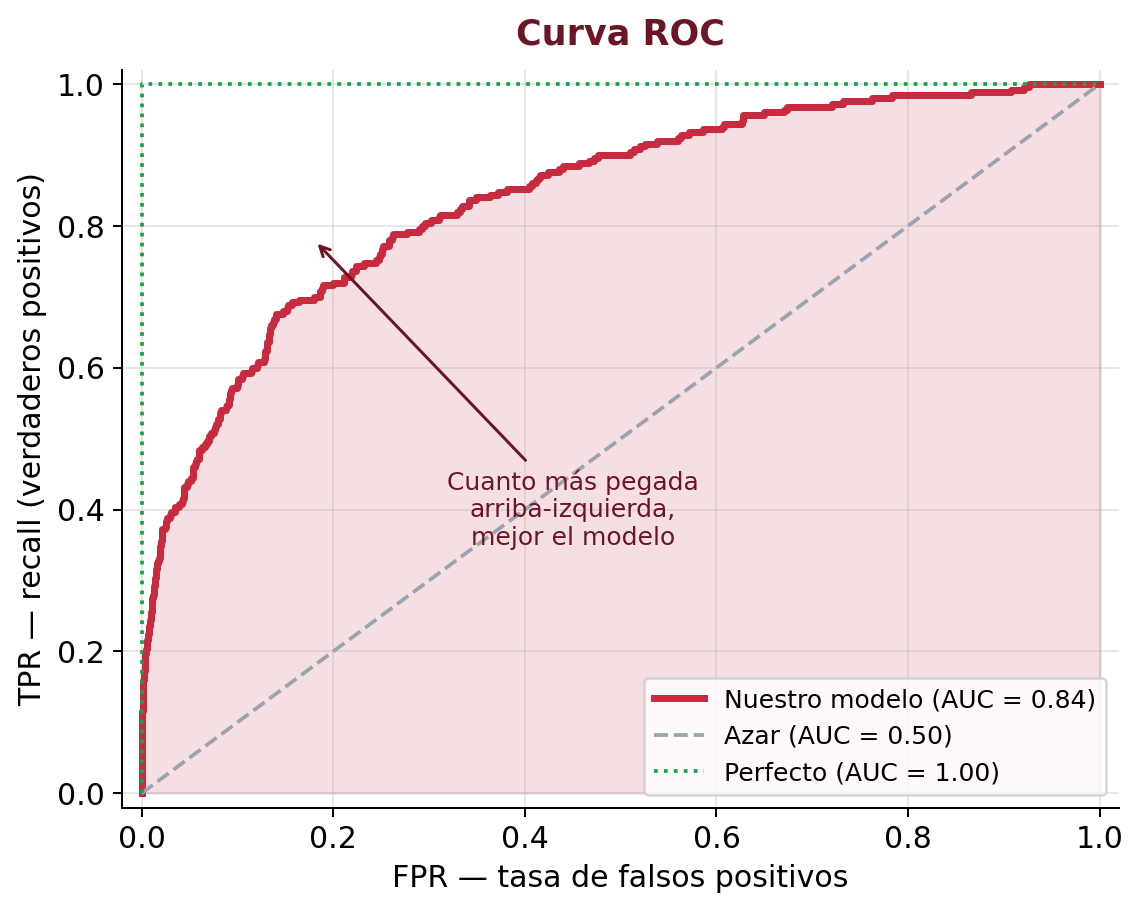
\includegraphics[width=0.5\textwidth]{fig_roc.png}
  \end{center}

  \vspace{-4pt}
  {\scriptsize\color{textMuted}
    \faLightbulb\hspace{4pt} \textbf{AUC} = área bajo la curva.
    1.0 = perfecto, 0.5 = azar, $\geq$ 0.8 se considera ``bueno''.
    Cuanto más arriba-izquierda esté la curva, mejor.}
\end{frame}

\begin{frame}[fragile,shrink=18]{Calcular y Graficar la Curva ROC}
  \vspace{-6pt}
  \begin{pyblock}
from sklearn.metrics import roc_curve, roc_auc_score
import plotly.express as px
import plotly.graph_objects as go

y_proba = modelo.predict_proba(X_test_s)[:, 1]
fpr, tpr, thresh = roc_curve(y_test, y_proba)
auc = roc_auc_score(y_test, y_proba)

fig = px.area(x=fpr, y=tpr,
    title=f"Curva ROC (AUC = {auc:.3f})",
    labels={"x": "FPR (1 - Especificidad)", "y": "TPR (Recall)"})
fig.add_shape(type="line", line=dict(dash="dash"),
              x0=0, x1=1, y0=0, y1=1)
fig.show()
  \end{pyblock}

  \vspace{4pt}
  {\scriptsize\color{textMuted}
    \faMousePointer\hspace{4pt} Con Plotly, al pasar el mouse se ven
    los valores exactos de cada punto (FPR, TPR).}
\end{frame}

% =============================================================================
%  BLOQUE B: CURVA PRECISION-RECALL (DETALLE COMPLETO)
% =============================================================================
\sectionframe{Curva Precision-Recall}{La correcta para desbalanceados}

\begin{frame}{¿Por Qué PR > ROC en Datos Desbalanceados?}
  \vspace{-4pt}
  {\footnotesize\color{arcaDark}\bfseries
    La curva ROC puede verse ``bonita'' incluso cuando el modelo es malo
    --- si el desbalance es fuerte.}

  \vspace{6pt}
  {\footnotesize
  \begin{itemize}\setlength{\itemsep}{4pt}
    \item[{\color{arcaRed}\scriptsize\faArrowRight}]
      El FPR tiene un denominador \textbf{enorme} (todos los sanos).
      Unos pocos falsos positivos ``se diluyen''.
    \item[{\color{arcaRed}\scriptsize\faArrowRight}]
      Ejemplo: 100 falsos positivos sobre 4861 sanos →
      FPR = 2\%. \textit{Parece bueno.}
    \item[{\color{arcaRed}\scriptsize\faArrowRight}]
      Pero si solo hay 249 positivos reales y detectamos 50,
      la \textbf{precisión} es 50/(50+100) = 33\%. \textit{Es malo.}
  \end{itemize}
  }

  \vspace{6pt}
  \begin{tcolorbox}[colback=arcaRed!8, colframe=arcaRed, boxrule=0.5pt,
    arc=2pt, left=6pt, right=6pt, top=4pt, bottom=4pt]
    {\scriptsize\color{arcaDark}
    \faKey\hspace{4pt}\textbf{Regla:} datos muy desbalanceados → usen
    \textbf{Precision-Recall}, no ROC. La PR se centra solo en la
    clase positiva (la que nos importa).}
  \end{tcolorbox}
\end{frame}

\begin{frame}[shrink=35]{Curva PR --- Los Ejes}
  \vspace{-4pt}
  \begin{center}
    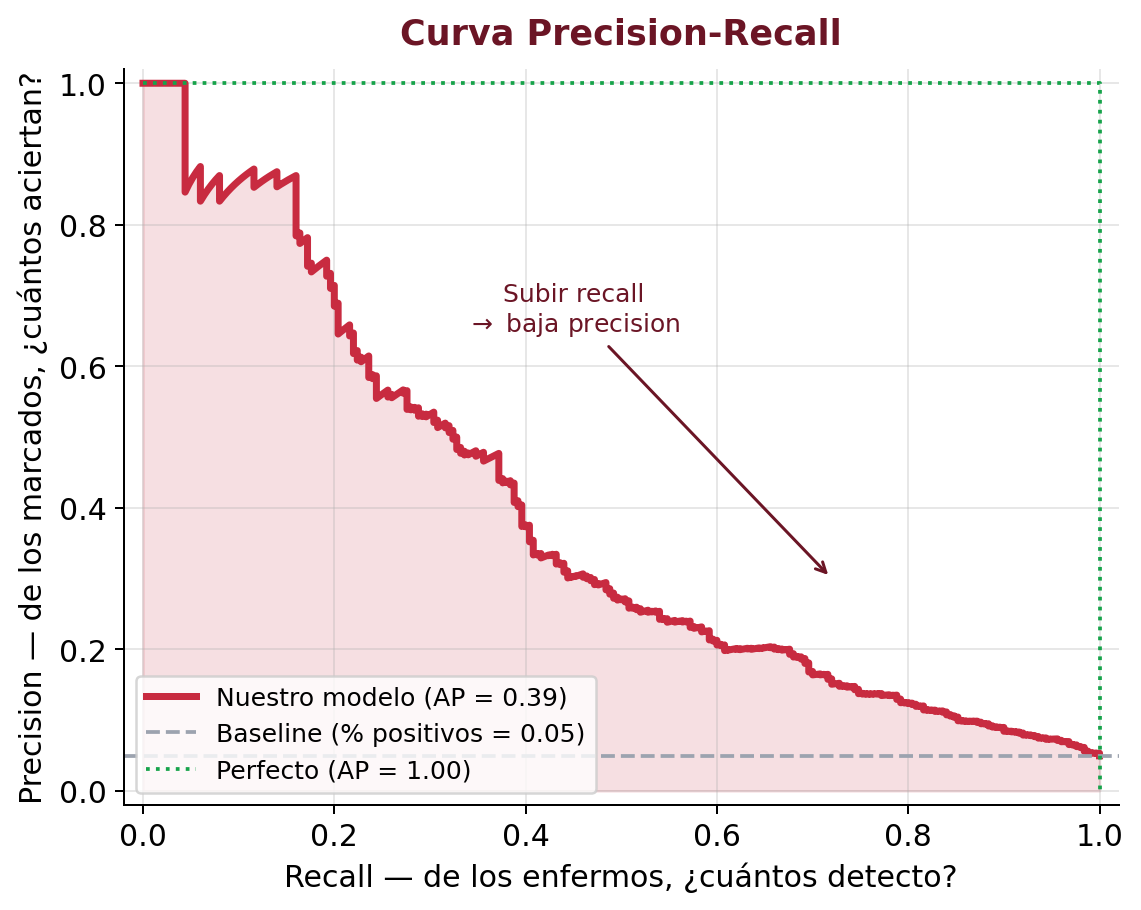
\includegraphics[width=0.5\textwidth]{fig_pr.png}
  \end{center}

  \vspace{-4pt}
  {\scriptsize\color{textMuted}
    \faLightbulb\hspace{4pt}
    \textbf{Precision} = VP / (VP + FP): de los que marqué, ¿cuántos son reales?
    \quad\textbf{Recall} = VP / (VP + FN): de los reales, ¿cuántos marqué?
    \quad\textbf{Trade-off}: subir uno baja el otro.}
\end{frame}

\begin{frame}{Cómo Se Calcula CADA Punto de la PR}
  \vspace{-4pt}
  {\footnotesize\color{arcaDark}\bfseries
    Misma receta que ROC, \textbf{cambia solo el eje}:}

  \vspace{4pt}
  {\footnotesize
  \begin{enumerate}\setlength{\itemsep}{3pt}
    \item Fijar un umbral $u$.
    \item \texttt{y\_pred = (proba >= u)}.
    \item Contar VP, FN, FP, VN.
    \item Calcular:
      $\text{Precision} = \dfrac{VP}{VP + FP}$, \quad
      $\text{Recall} = \dfrac{VP}{VP + FN}$
    \item Graficar el punto $(\text{Recall}, \text{Precision})$.
  \end{enumerate}
  }

  \vspace{4pt}
  \begin{tcolorbox}[colback=arcaRed!8, colframe=arcaRed, boxrule=0.5pt,
    arc=2pt, left=6pt, right=6pt, top=4pt, bottom=4pt]
    {\scriptsize\color{arcaDark}
    \faKey\hspace{4pt}\textbf{Diferencia con ROC:} el eje X ahora es el mismo
    (Recall = TPR), pero el Y es \textbf{Precision} (no FPR). La precisión
    \textit{ignora los verdaderos negativos} → se concentra en la clase positiva.}
  \end{tcolorbox}
\end{frame}

\begin{frame}[shrink=42]{3 Umbrales = 3 Puntos en la Curva PR}
  \vspace{-4pt}
  \begin{center}
    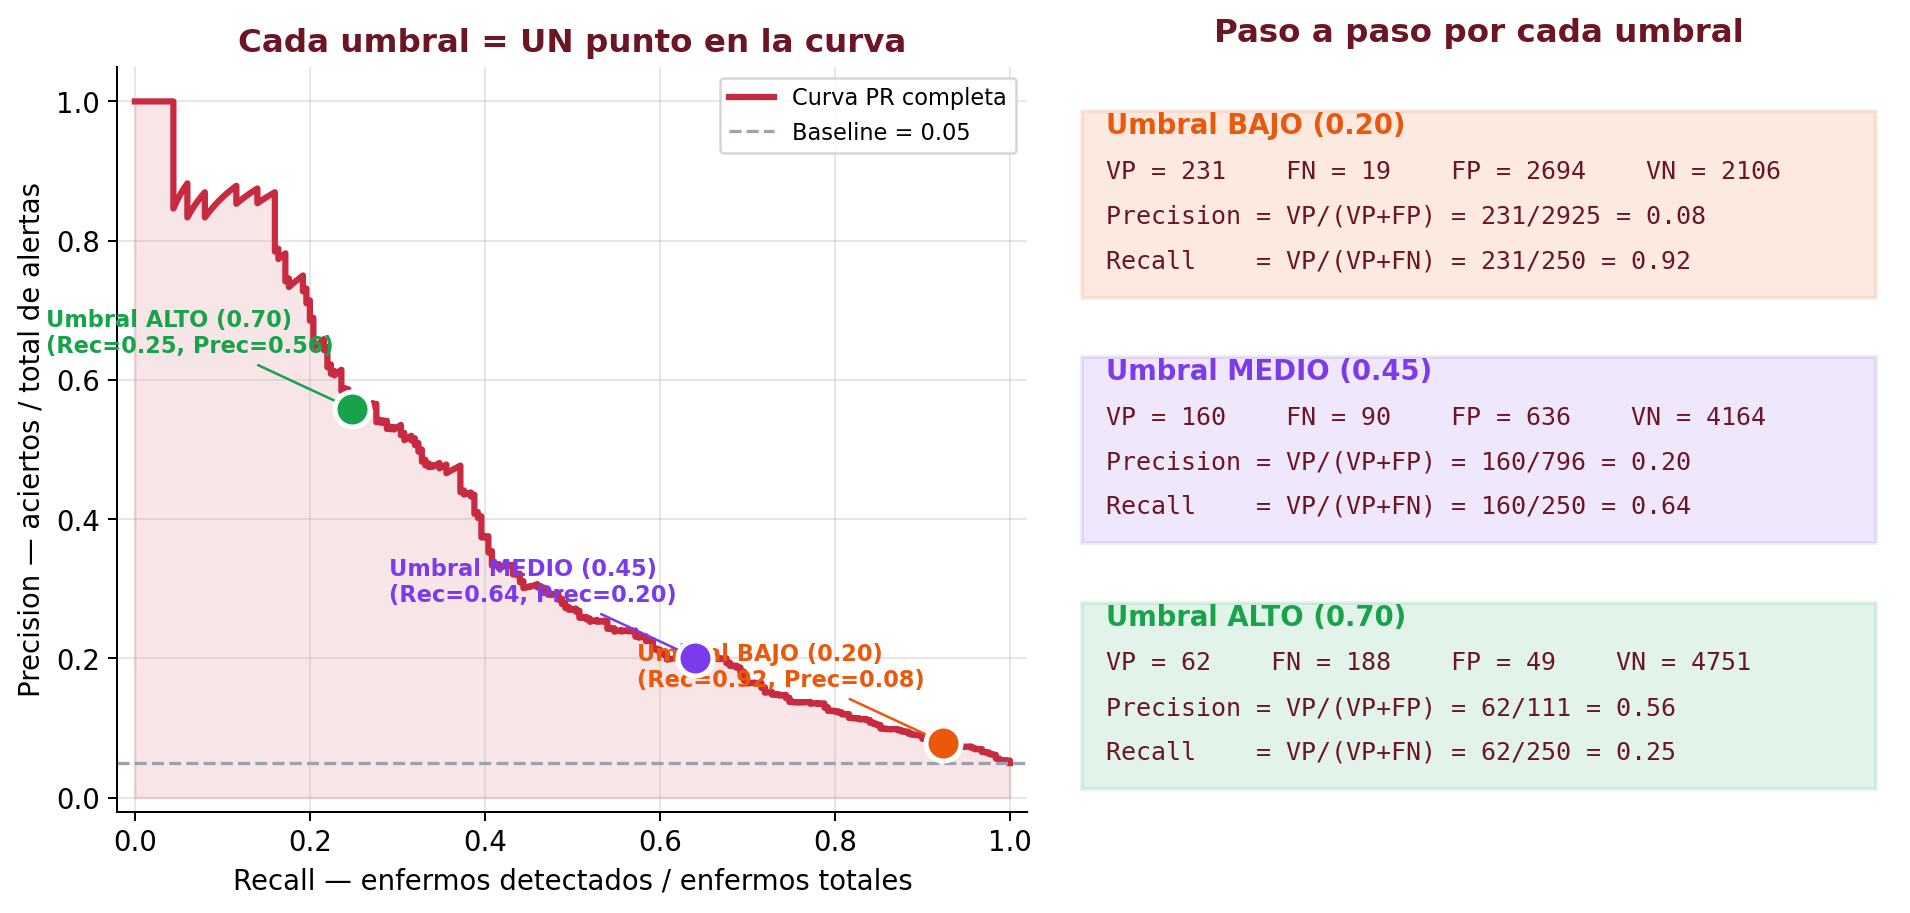
\includegraphics[width=0.82\textwidth]{fig_pr_puntos.png}
  \end{center}

  \vspace{-2pt}
  {\scriptsize\color{textMuted}
    \faLightbulb\hspace{4pt} Con \textbf{umbral alto} (verde) la precisión
    sube pero el recall cae → detectamos pocos pero acertamos. Con
    \textbf{umbral bajo} (naranja) es al revés.}
\end{frame}

\begin{frame}[shrink=15]{¿Cómo Se Calcula el AP (Average Precision)?}
  \vspace{-4pt}
  {\footnotesize\color{arcaDark}\bfseries
    AP = área bajo la curva PR. Pero sklearn lo calcula \textbf{distinto} al AUC.}

  \vspace{6pt}
  {\footnotesize
  \begin{itemize}\setlength{\itemsep}{4pt}
    \item[{\color{arcaRed}\scriptsize\faArrowRight}]
      \textbf{Promedio ponderado} de la precisión en cada punto, pesado por
      cuánto subió el recall:
      $$\text{AP} = \sum_n (R_n - R_{n-1}) \cdot P_n$$
    \item[{\color{arcaRed}\scriptsize\faArrowRight}]
      Es una \textbf{suma de rectángulos} (no trapecios como AUC) --- esto
      evita sobrestimar la curva, que es ``escalonada'' en PR.
    \item[{\color{arcaRed}\scriptsize\faArrowRight}]
      Un modelo \textbf{aleatorio} tiene AP = proporción de positivos
      (en stroke, AP aleatorio $\approx$ 0.05).
  \end{itemize}
  }

  \vspace{4pt}
  \begin{tcolorbox}[colback=codeGreen!8, colframe=codeGreen, boxrule=0.5pt,
    arc=2pt, left=6pt, right=6pt, top=4pt, bottom=4pt]
    {\scriptsize\color{arcaDark}
    \faLightbulb\hspace{4pt} Lee: un AP de 0.30 en datos con 5\% de positivos
    significa que el modelo es \textbf{6x mejor que el azar} al rankear
    los positivos arriba.}
  \end{tcolorbox}
\end{frame}

\begin{frame}[fragile,shrink=18]{Calcular y Graficar la Curva PR}
  \vspace{-6pt}
  \begin{pyblock}
from sklearn.metrics import precision_recall_curve, average_precision_score

prec, rec, thr = precision_recall_curve(y_test, y_proba)
ap = average_precision_score(y_test, y_proba)

fig = px.area(x=rec, y=prec,
    title=f"Curva Precision-Recall (AP = {ap:.3f})",
    labels={"x": "Recall", "y": "Precision"})

# Linea de baseline (prevalencia)
fig.add_hline(y=y_test.mean(), line_dash="dash",
              annotation_text="baseline (% positivos)")
fig.show()
  \end{pyblock}

  \vspace{4pt}
  {\scriptsize\color{textMuted}
  \begin{itemize}\setlength{\itemsep}{3pt}
    \item[{\color{arcaRed}\scriptsize\faArrowRight}]
      \textbf{AP} (Average Precision): área bajo la curva PR.
      En datos muy desbalanceados, un AP de 0.30 ya es \textit{notable}
      (baseline es 0.05).
  \end{itemize}
  }
\end{frame}

% =============================================================================
%  BLOQUE C: UMBRAL ÓPTIMO
% =============================================================================
\sectionframe{Umbral Óptimo}{Llevando la evaluación al negocio}

\begin{frame}{El Costo del Error NO Es Simétrico}
  \vspace{-4pt}
  {\footnotesize\color{arcaDark}\bfseries
    En un hospital:}

  \vspace{6pt}
  \begin{columns}[T]
    \begin{column}{0.48\textwidth}
      \begin{tcolorbox}[colback=arcaRed!10, colframe=arcaRed, boxrule=0.5pt,
        arc=2pt, title={\small\color{white}\bfseries\faHeartbeat\ Falso Negativo}]
        {\scriptsize
        Paciente \textbf{tiene} riesgo, el modelo dice que no.
        \vspace{3pt}
        \begin{itemize}\setlength{\itemsep}{2pt}
          \item Costo: \textbf{vida humana}
          \item Valor: \$\$\$\$\$
        \end{itemize}
        }
      \end{tcolorbox}
    \end{column}
    \begin{column}{0.48\textwidth}
      \begin{tcolorbox}[colback=codeOrange!10, colframe=codeOrange, boxrule=0.5pt,
        arc=2pt, title={\small\color{white}\bfseries\faStethoscope\ Falso Positivo}]
        {\scriptsize
        Paciente \textbf{no tiene} riesgo, el modelo dice que sí.
        \vspace{3pt}
        \begin{itemize}\setlength{\itemsep}{2pt}
          \item Costo: chequeo adicional
          \item Valor: \$
        \end{itemize}
        }
      \end{tcolorbox}
    \end{column}
  \end{columns}

  \vspace{8pt}
  {\footnotesize\color{arcaDark}
    \faArrowRight\hspace{4pt} En medicina, preferimos \textbf{recall alto}
    aunque la precisión baje. Esto implica \textbf{bajar el umbral}
    por debajo de 0.5.}
\end{frame}

\begin{frame}[fragile,shrink=28]{Explorar Umbrales}
  \vspace{-6pt}
  \begin{pyblock}
import numpy as np
import pandas as pd

umbrales = np.arange(0.1, 0.9, 0.05)
resultados = []
for u in umbrales:
    y_pred_u = (y_proba >= u).astype(int)
    resultados.append({
        "umbral": u,
        "precision": precision_score(y_test, y_pred_u, zero_division=0),
        "recall":    recall_score(y_test, y_pred_u),
    })
df_u = pd.DataFrame(resultados)

fig = px.line(df_u.melt(id_vars="umbral"),
              x="umbral", y="value", color="variable",
              title="Precision y Recall vs Umbral")
fig.show()
  \end{pyblock}
\end{frame}

\begin{frame}{Elegir el Umbral con Lógica de Negocio}
  \vspace{-4pt}
  {\footnotesize\color{arcaDark}\bfseries
    Tres estrategias comunes:}

  \vspace{6pt}
  {\footnotesize
  \begin{enumerate}\setlength{\itemsep}{6pt}
    \item[{\color{arcaRed}\bfseries 1.}]
      \textbf{F1 máximo}: balance precision-recall.\\
      \texttt{f1 = 2 * P * R / (P + R)} --- útil cuando no hay preferencia clara.
    \item[{\color{arcaRed}\bfseries 2.}]
      \textbf{Recall mínimo}: ``detecta al menos 80\% de los ACV''.
      Buscar el umbral más alto que cumpla → menos falsos positivos posibles.
    \item[{\color{arcaRed}\bfseries 3.}]
      \textbf{Costo esperado}: multiplicar errores por su costo y minimizar.\\
      \texttt{costo = FN * c\_FN + FP * c\_FP}
  \end{enumerate}
  }

  \vspace{6pt}
  \begin{tcolorbox}[colback=arcaGray, colframe=arcaRed, boxrule=0.5pt, arc=2pt,
    left=6pt, right=6pt, top=4pt, bottom=4pt]
    {\scriptsize\color{arcaDark}
    \faLightbulb\hspace{4pt} Si un FN cuesta \$10.000 (tratamiento tardío)
    y un FP cuesta \$200 (un chequeo), la razón es 50:1. El umbral
    óptimo será \textbf{mucho más bajo} que 0.5.}
  \end{tcolorbox}
\end{frame}

\begin{frame}[fragile,shrink=25]{Caso de Negocio: Umbral por Costo}
  \vspace{-6pt}
  \begin{pyblock}
COSTO_FN = 10_000   # no detectar ACV
COSTO_FP = 200      # falsa alarma

from sklearn.metrics import confusion_matrix
costos = []
for u in umbrales:
    y_pred_u = (y_proba >= u).astype(int)
    tn, fp, fn, tp = confusion_matrix(y_test, y_pred_u).ravel()
    costos.append({"umbral": u,
                   "costo": fn*COSTO_FN + fp*COSTO_FP})

df_c = pd.DataFrame(costos)
u_opt = df_c.loc[df_c["costo"].idxmin(), "umbral"]
print(f"Umbral optimo: {u_opt:.2f}")

px.line(df_c, x="umbral", y="costo",
        title=f"Costo esperado (optimo: {u_opt:.2f})").show()
  \end{pyblock}
\end{frame}

\begin{frame}[shrink=5]{Ejercicio 1: Tu Curva ROC y PR}
  \vspace{-4pt}
  {\footnotesize\color{arcaDark}\bfseries
    \faClock\hspace{4pt} 15 minutos --- en el notebook:}

  \vspace{6pt}
  {\footnotesize
  \begin{enumerate}\setlength{\itemsep}{4pt}
    \item Carguen el dataset de stroke y preparen X, y.
    \item Train/test split con \texttt{stratify=y}.
    \item Entrenen logística con \texttt{class\_weight="balanced"}.
    \item Grafiquen la \textbf{curva ROC} con Plotly. Reporten AUC.
    \item Grafiquen la \textbf{curva PR}. Reporten AP.
    \item Prueben 5 umbrales y calculen el costo con FN=\$10\,000, FP=\$200.
    \item ¿Qué umbral eligirían si un FN cuesta 50x más que un FP?
  \end{enumerate}
  }
\end{frame}

% =============================================================================
%  BLOQUE D: ÁRBOLES DE DECISIÓN — INTUICIÓN
% =============================================================================
\sectionframe{Árboles de Decisión}{El modelo que se explica solo}

\begin{frame}{La Intuición: 20 Preguntas}
  \vspace{-4pt}
  {\footnotesize\color{arcaDark}\bfseries
    ¿Conocen el juego de ``20 preguntas''? Alguien piensa en algo y tú
    preguntas sí/no hasta adivinarlo.}

  \vspace{6pt}
  {\footnotesize
  \begin{itemize}\setlength{\itemsep}{4pt}
    \item[{\color{arcaRed}\scriptsize\faArrowRight}]
      Un árbol de decisión hace \textbf{exactamente eso} con los datos.
    \item[{\color{arcaRed}\scriptsize\faArrowRight}]
      En cada nodo, hace una pregunta sobre \textbf{una variable}:
      ``¿edad $>$ 60?'', ``¿glucosa $>$ 200?''
    \item[{\color{arcaRed}\scriptsize\faArrowRight}]
      Según la respuesta, va por una rama u otra.
    \item[{\color{arcaRed}\scriptsize\faArrowRight}]
      Al final (en las \textbf{hojas}) da su predicción.
  \end{itemize}
  }

  \vspace{6pt}
  \begin{tcolorbox}[colback=codeGreen!8, colframe=codeGreen, boxrule=0.5pt, arc=2pt,
    left=6pt, right=6pt, top=4pt, bottom=4pt]
    {\scriptsize\color{arcaDark}
    \faLightbulb\hspace{4pt}\textbf{Ventaja clave:} puedes \textit{leer} el
    árbol y explicarle a un gerente o médico por qué el modelo decidió algo.
    Con logística no es tan fácil.}
  \end{tcolorbox}
\end{frame}

\begin{frame}[shrink=18]{Un Árbol para Predicción de ACV}
  \vspace{-4pt}
  \begin{center}
    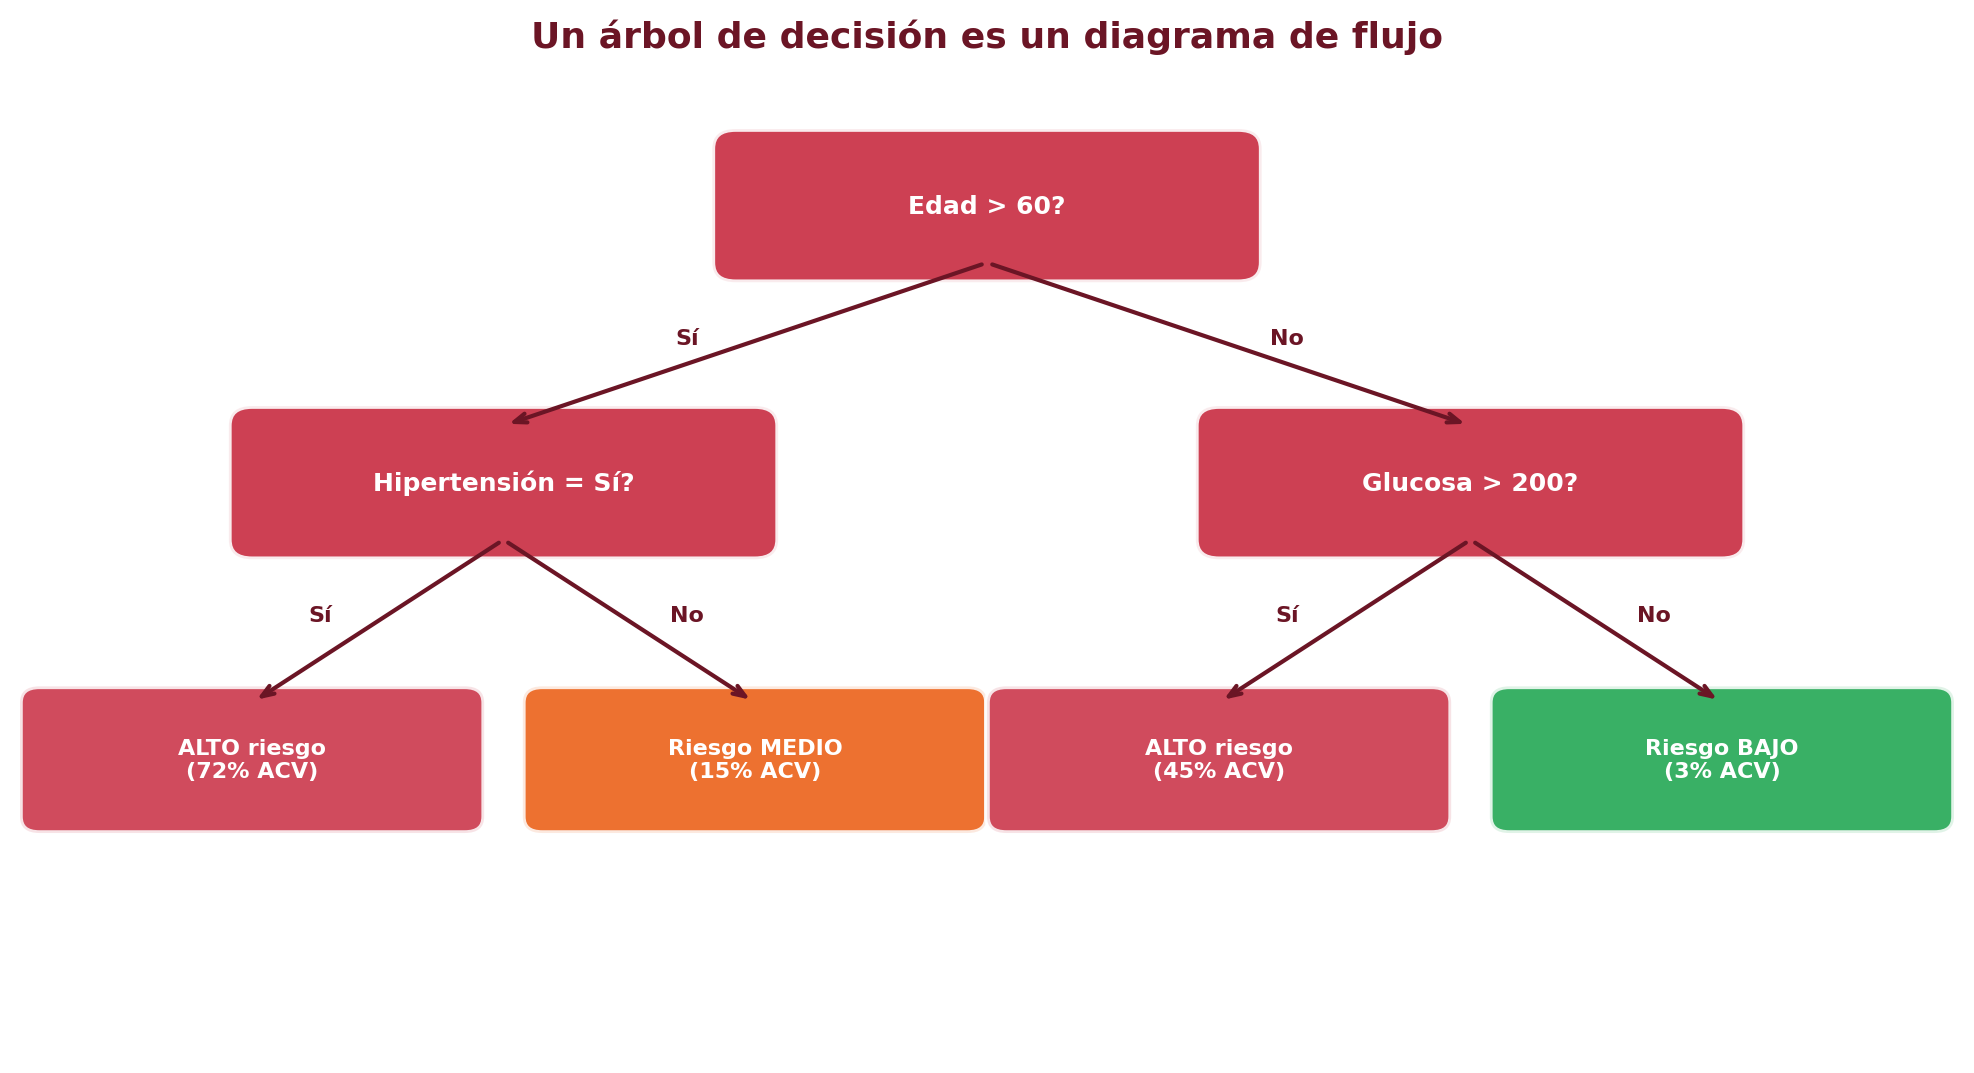
\includegraphics[width=0.9\textwidth]{fig_20preguntas.png}
  \end{center}

  \vspace{-2pt}
  {\scriptsize\color{textMuted}
    \faLightbulb\hspace{4pt} Cada caja es una \textbf{pregunta}.
    Cada hoja es una \textbf{predicción}. El camino desde la raíz
    hasta la hoja es la \textbf{explicación} de por qué el modelo decidió.}
\end{frame}

\begin{frame}{Vocabulario del Árbol}
  \vspace{-4pt}
  \begin{center}
  \begin{tikzpicture}[
    every node/.style={font=\footnotesize},
    node distance=0.6cm,
    nodo/.style={rectangle, rounded corners=3pt, draw=arcaRed, fill=arcaRed!10,
                 minimum width=2.5cm, minimum height=0.6cm, align=center,
                 font=\scriptsize\bfseries\color{arcaDark}},
    hoja/.style={rectangle, rounded corners=3pt, draw=codeGreen, fill=codeGreen!15,
                 minimum width=1.5cm, minimum height=0.5cm, align=center,
                 font=\scriptsize\bfseries\color{arcaDark}},
  ]
    \node[nodo] (root) at (0, 3.5) {Edad $>$ 60?};
    \node[nodo] (l1) at (-3, 2) {Glucosa $>$ 200?};
    \node[nodo] (r1) at (3, 2) {Hipertensión?};

    \node[hoja] (ll) at (-4.5, 0.5) {No ACV};
    \node[hoja] (lr) at (-1.5, 0.5) {ACV};
    \node[hoja] (rl) at (1.5, 0.5) {ACV};
    \node[hoja] (rr) at (4.5, 0.5) {No ACV};

    \draw[->, arcaDark, thick] (root) -- node[left, font=\tiny] {Sí} (l1);
    \draw[->, arcaDark, thick] (root) -- node[right, font=\tiny] {No} (r1);
    \draw[->, arcaDark, thick] (l1) -- node[left, font=\tiny] {No} (ll);
    \draw[->, arcaDark, thick] (l1) -- node[right, font=\tiny] {Sí} (lr);
    \draw[->, arcaDark, thick] (r1) -- node[left, font=\tiny] {Sí} (rl);
    \draw[->, arcaDark, thick] (r1) -- node[right, font=\tiny] {No} (rr);

    % Labels
    \node[font=\scriptsize\color{arcaRed}, right] at (1.5, 3.5) {\faArrowLeft\ \textbf{Raíz} (root)};
    \node[font=\scriptsize\color{arcaDark}, left] at (-5.2, 2) {\textbf{Nodo interno} \faArrowRight};
    \node[font=\scriptsize\color{codeGreen}, right] at (5.2, 0.5) {\faArrowLeft\ \textbf{Hoja} (leaf)};

    \draw[decorate, decoration={brace, amplitude=5pt, raise=3pt}, arcaDark]
      (-4.5, -0.1) -- (4.5, -0.1)
      node[midway, below, yshift=-8pt, font=\scriptsize\color{arcaDark}]
      {\textbf{Profundidad} (depth) = número de niveles de preguntas};
  \end{tikzpicture}
  \end{center}

  \vspace{4pt}
  {\scriptsize\color{textMuted}
    \faArrowRight\hspace{4pt} \textbf{Raíz}: primera pregunta.
    \textbf{Nodos internos}: preguntas intermedias.
    \textbf{Hojas}: predicción final.
    \textbf{Profundidad}: cuántas preguntas hay del inicio al final.}
\end{frame}

\begin{frame}{¿Por Qué Necesitamos Otro Modelo?}
  \vspace{-4pt}
  {\footnotesize\color{arcaDark}\bfseries
    La logística asume que la relación entre variables y riesgo es
    una \textbf{línea recta}. Pero la vida real no siempre es lineal.}

  \vspace{6pt}
  {\footnotesize
  \begin{itemize}\setlength{\itemsep}{5pt}
    \item[{\color{codeBlue}\scriptsize\faArrowRight}]
      \textbf{Logística dice:} ``por cada año más de edad, el riesgo
      sube \textit{la misma cantidad}''. Siempre proporcional.
    \item[{\color{arcaRed}\scriptsize\faArrowRight}]
      \textbf{Realidad:} el riesgo de ACV no sube igual de 20 a 30
      que de 60 a 70. Hay \textbf{saltos}, \textbf{umbrales},
      \textbf{combinaciones} que la línea recta no puede capturar.
    \item[{\color{arcaRed}\scriptsize\faArrowRight}]
      Ejemplo: ``edad $>$ 60 \textbf{Y} hipertensión = riesgo alto''.
      Esa \textit{interacción} la logística no la ve, pero el árbol sí.
  \end{itemize}
  }

  \vspace{6pt}
  \begin{tcolorbox}[colback=arcaGray, colframe=arcaRed, boxrule=0.5pt, arc=2pt,
    left=6pt, right=6pt, top=4pt, bottom=4pt]
    {\scriptsize\color{arcaDark}
    \faLightbulb\hspace{4pt}\textbf{Analogía:} la logística es como trazar
    una frontera con una \textit{regla}. El árbol es como trazar la frontera
    con \textit{tijeras} --- puede recortar formas complejas.}
  \end{tcolorbox}
\end{frame}

\begin{frame}[shrink=22]{Un Problema que la Logística NO Puede Resolver}
  \vspace{-4pt}
  \begin{center}
    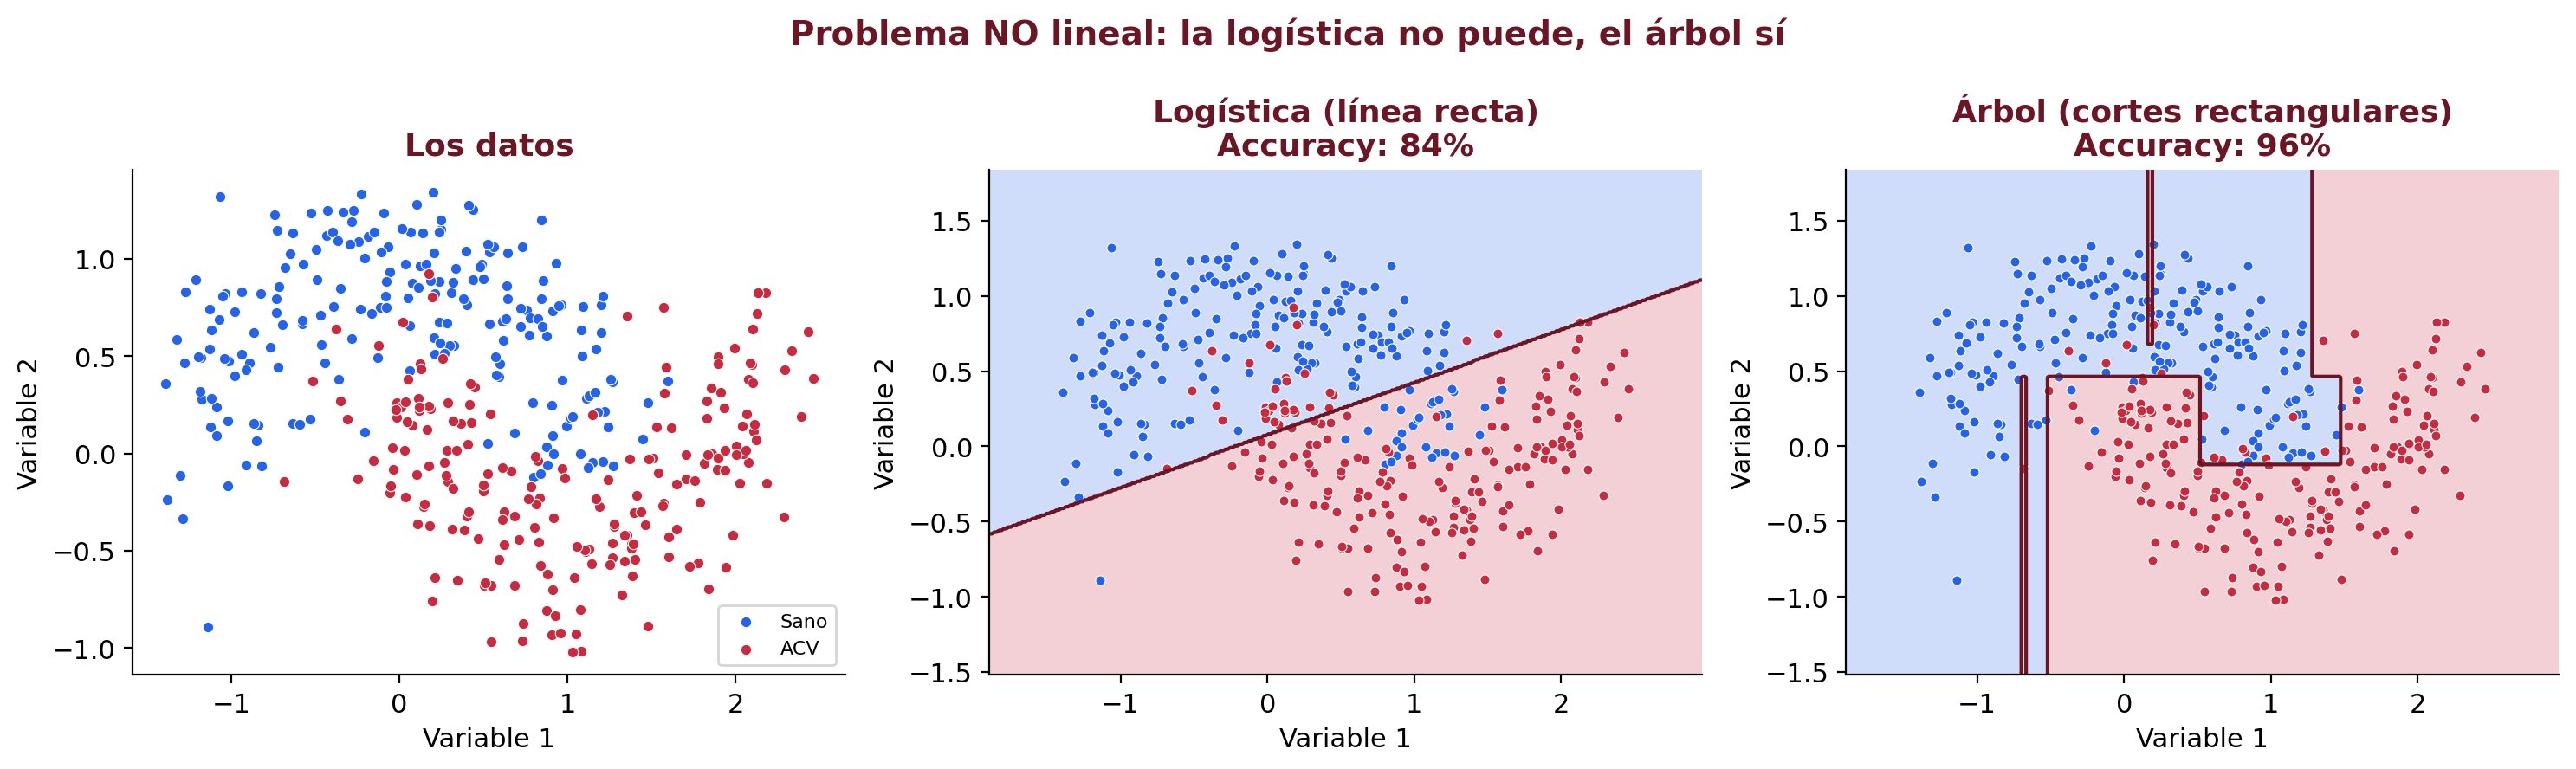
\includegraphics[width=0.95\textwidth]{fig_frontera.png}
  \end{center}

  \vspace{-2pt}
  {\scriptsize\color{textMuted}
    \faLightbulb\hspace{4pt} \textbf{Izquierda:} los datos (dos medialunas
    entrelazadas). \textbf{Centro:} la logística intenta separar con una línea
    recta --- imposible, falla. \textbf{Derecha:} el árbol hace cortes
    rectangulares y los separa bien. Cuando la relación no es lineal,
    el árbol gana.}
\end{frame}

\begin{frame}{Logística vs Árbol --- Dos Formas de Pensar}
  \vspace{-4pt}
  {\footnotesize\color{arcaDark}\bfseries
    Piénsenlo como dos médicos con estilos distintos:}

  \vspace{6pt}
  {\scriptsize
  \begin{tabular}{@{}p{3.5cm}p{4.5cm}p{4.5cm}@{}}
    \toprule
     & \textbf{\color{codeBlue}Dr. Logística} & \textbf{\color{arcaRed}Dr. Árbol} \\
    \midrule
    \textbf{Cómo piensa} & ``Peso cada factor, los sumo, y si pasan cierto nivel → riesgo.'' & ``¿Tiene más de 60? Sí. ¿Hipertenso? Sí → riesgo alto.'' \\
    \textbf{Lo que ve} & Todo a la vez (suma ponderada). & Una cosa a la vez (preguntas). \\
    \textbf{Explicación al paciente} & ``Su combinación de factores da un 73\%.'' & ``Porque es mayor de 60 e hipertenso.'' \\
    \textbf{Debilidad} & Asume que todo es proporcional. & Puede sobrecomplicarse y memorizar. \\
    \bottomrule
  \end{tabular}
  }

  \vspace{6pt}
  {\scriptsize\color{textMuted}
    \faLightbulb\hspace{4pt} Ninguno es ``mejor''. Son \textbf{complementarios}.
    Hoy los entrenamos ambos y elegimos con datos.}
\end{frame}

% =============================================================================
%  BLOQUE E: GINI Y ENTROPÍA
% =============================================================================
\sectionframe{Gini}{Cómo el árbol elige las preguntas}

\begin{frame}{La Bolsa de Caramelos --- Intuición de Gini}
  \vspace{-4pt}
  {\footnotesize\color{arcaDark}\bfseries
    Imaginen que tienen una bolsa con caramelos rojos y azules.
    Meten la mano \textbf{sin ver} y sacan dos al azar.}

  \vspace{6pt}
  {\footnotesize
  \begin{itemize}\setlength{\itemsep}{5pt}
    \item[{\color{codeGreen}\scriptsize\faArrowRight}]
      Si la bolsa tiene \textbf{100 rojos y 0 azules}: siempre sacan
      dos rojos. La bolsa es \textbf{pura}. No hay sorpresa.
    \item[{\color{codeOrange}\scriptsize\faArrowRight}]
      Si tiene \textbf{50 rojos y 50 azules}: máxima incertidumbre.
      No saben qué va a salir. La bolsa está \textbf{mezclada}.
    \item[{\color{arcaRed}\scriptsize\faArrowRight}]
      \textbf{Gini mide exactamente eso}: la probabilidad de que dos
      caramelos al azar sean de clase \textit{distinta}.
  \end{itemize}
  }

  \vspace{6pt}
  \begin{tcolorbox}[colback=arcaGray, colframe=arcaRed, boxrule=0.5pt, arc=2pt,
    left=6pt, right=6pt, top=4pt, bottom=4pt]
    {\scriptsize\color{arcaDark}
    \faKey\hspace{4pt}\textbf{Gini = 0}: bolsa pura (todos iguales).
    \textbf{Gini = 0.5}: máxima mezcla (mitad y mitad).
    El árbol busca cortes que hagan las bolsas lo más \textbf{puras} posible.}
  \end{tcolorbox}
\end{frame}

\begin{frame}[shrink=15]{Gini en Números}
  \vspace{-4pt}
  {\footnotesize\color{arcaDark}\bfseries
    La fórmula es simple: Gini = 1 menos la suma de cada proporción al cuadrado.}

  \vspace{6pt}
  \begin{center}
    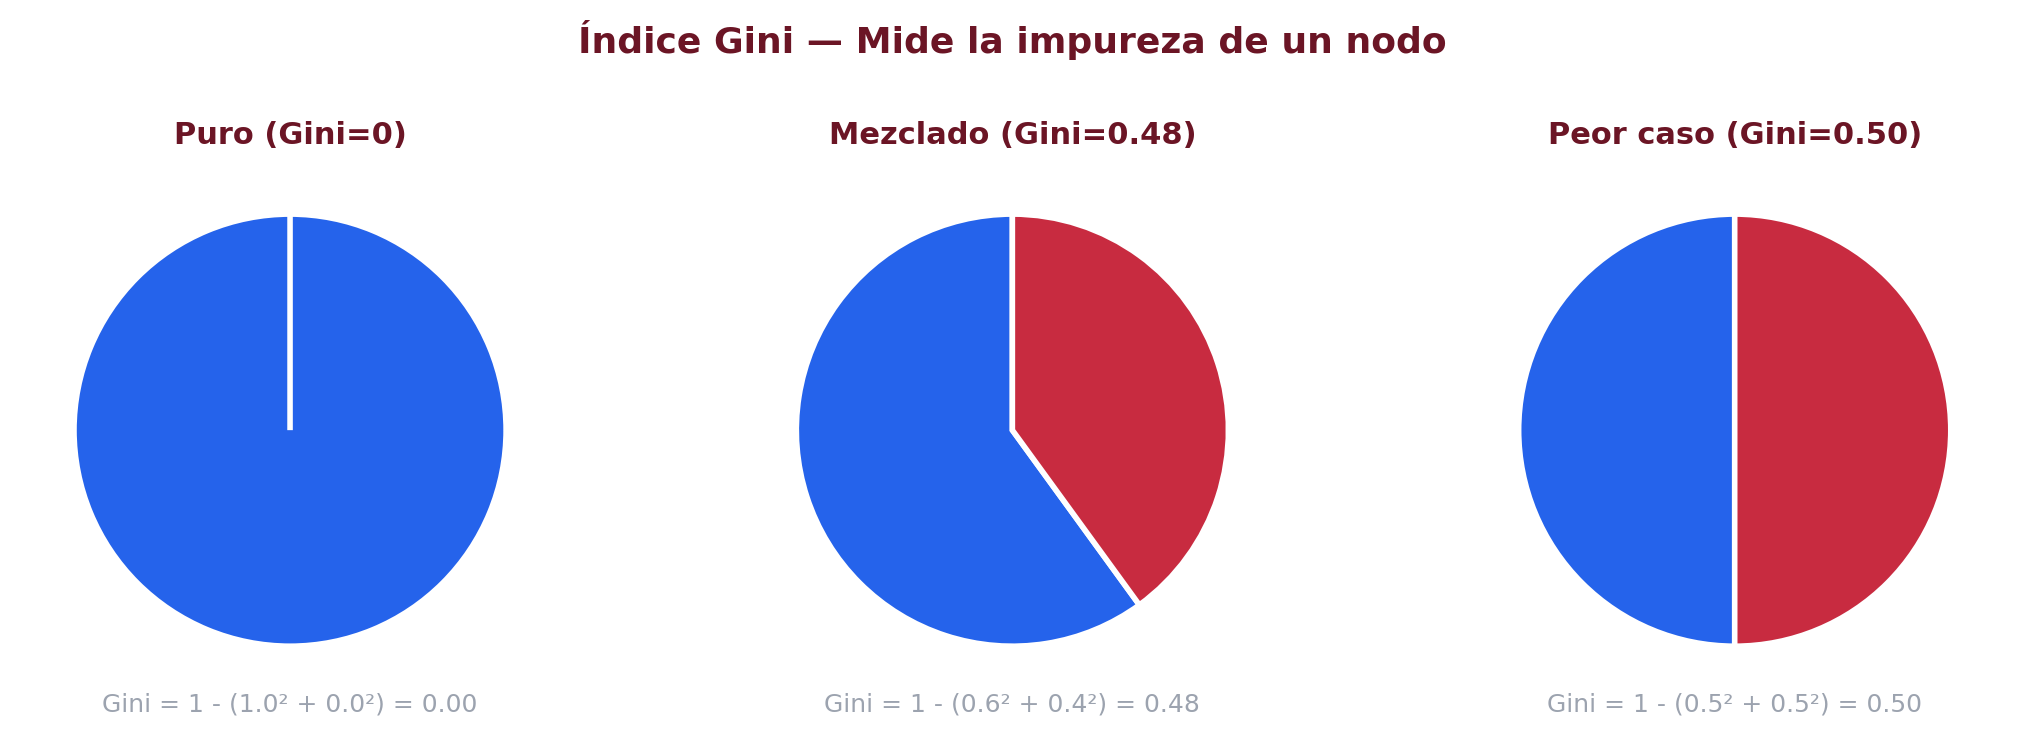
\includegraphics[width=0.85\textwidth]{fig_gini.png}
  \end{center}

  \vspace{2pt}
  {\scriptsize
  \begin{itemize}\setlength{\itemsep}{3pt}
    \item[{\color{arcaRed}\scriptsize\faArrowRight}]
      $\text{Gini} = 1 - (p_{\text{clase1}}^2 + p_{\text{clase2}}^2)$
    \item[{\color{arcaRed}\scriptsize\faArrowRight}]
      Bolsa de 100\% rojos: $1 - (1.0^2 + 0.0^2) = 0$ → pura.
    \item[{\color{arcaRed}\scriptsize\faArrowRight}]
      Bolsa de 50/50: $1 - (0.5^2 + 0.5^2) = 0.5$ → máxima mezcla.
    \item[{\color{arcaRed}\scriptsize\faArrowRight}]
      El árbol elige el corte que \textbf{más reduzca} el Gini de los hijos.
  \end{itemize}
  }
\end{frame}

\begin{frame}{¿De Dónde Sale el ``60'' en ``Edad $>$ 60''?}
  \vspace{-4pt}
  {\footnotesize\color{arcaDark}\bfseries
    El umbral \textbf{no es arbitrario}. El árbol lo encuentra
    probando todos los valores posibles.}

  \vspace{6pt}
  {\footnotesize
  \begin{itemize}\setlength{\itemsep}{5pt}
    \item[{\color{arcaRed}\scriptsize\faArrowRight}]
      Si los pacientes tienen edades 23, 31, 45, 52, 58, 63, 71, 78\ldots
    \item[{\color{arcaRed}\scriptsize\faArrowRight}]
      El árbol prueba cortar en \textbf{cada punto medio}:
      27, 38, 48.5, 55, 60.5, 67, 74.5\ldots
    \item[{\color{arcaRed}\scriptsize\faArrowRight}]
      Para \textbf{cada} corte calcula el Gini de los dos grupos resultantes.
    \item[{\color{arcaRed}\scriptsize\faArrowRight}]
      Elige el corte que produce los grupos \textbf{más puros}.
  \end{itemize}
  }

  \vspace{6pt}
  \begin{tcolorbox}[colback=arcaGray, colframe=arcaRed, boxrule=0.5pt, arc=2pt,
    left=6pt, right=6pt, top=4pt, bottom=4pt]
    {\scriptsize\color{arcaDark}
    \faKey\hspace{4pt}\textbf{Fuerza bruta:} el árbol prueba TODAS las
    variables × TODOS los posibles puntos de corte. No adivina ---
    evalúa cada opción y elige la mejor. Por eso es tan bueno encontrando
    patrones, pero también por eso puede memorizar si no lo podamos.}
  \end{tcolorbox}
\end{frame}

\begin{frame}{Cómo Elige la Variable Y el Umbral --- Ejemplo}
  \vspace{-4pt}
  {\footnotesize\color{arcaDark}\bfseries
    100 pacientes (80 sanos, 20 ACV). El árbol evalúa cada opción:}

  \vspace{6pt}
  {\footnotesize
  \begin{enumerate}\setlength{\itemsep}{4pt}
    \item[{\color{arcaRed}\bfseries 1.}]
      Gini actual: $1 - (0.8^2 + 0.2^2) = 0.32$ (bastante mezclado).
    \item[{\color{arcaRed}\bfseries 2.}]
      Prueba ``\textbf{edad $>$ 55}'': Gini ponderado = 0.330
    \item[{\color{arcaRed}\bfseries 3.}]
      Prueba ``\textbf{edad $>$ 60}'': Gini ponderado = 0.316 \hfill ← mejor
    \item[{\color{arcaRed}\bfseries 4.}]
      Prueba ``\textbf{edad $>$ 65}'': Gini ponderado = 0.325
    \item[{\color{arcaRed}\bfseries 5.}]
      Prueba ``\textbf{glucosa $>$ 200}'': Gini ponderado = 0.335
    \item[{\color{arcaRed}\bfseries 6.}]
      Prueba ``\textbf{bmi $>$ 30}'': Gini ponderado = 0.318
    \item[] \ldots y así para \textbf{cada variable y cada valor}.
  \end{enumerate}
  }

  \vspace{4pt}
  {\scriptsize\color{textMuted}
    \faLightbulb\hspace{4pt} Gana ``edad $>$ 60'' porque tiene el \textbf{Gini
    más bajo} (0.316). El ``60'' no lo decidió un humano --- lo encontró el
    algoritmo. sklearn hace este cálculo automáticamente.}
\end{frame}

% =============================================================================
%  BLOQUE F: DECISIONTREECLASSIFIER EN SKLEARN
% =============================================================================
\sectionframe{DecisionTreeClassifier}{Construir un árbol en Python}

\begin{frame}[fragile,shrink=18]{Tu Primer Árbol --- 4 Líneas}
  \vspace{-6pt}
  \begin{pyblock}
from sklearn.tree import DecisionTreeClassifier

arbol = DecisionTreeClassifier(random_state=42)
arbol.fit(X_train, y_train)

print(f"Accuracy train: {arbol.score(X_train, y_train):.3f}")
print(f"Accuracy test:  {arbol.score(X_test, y_test):.3f}")
  \end{pyblock}

  \vspace{4pt}
  \begin{outputblock}
Accuracy train: 1.000
Accuracy test:  0.906
  \end{outputblock}

  \vspace{4pt}
  {\scriptsize\color{arcaRed}
    \faExclamationTriangle\hspace{4pt}\textbf{¡Atención!} El accuracy de train
    es \textbf{1.0} (perfecto). El modelo \textit{memorizó} los datos.
    Esto se llama \textbf{overfitting}.}
\end{frame}

\begin{frame}[fragile,shrink=10]{¿Qué Pasó? --- El Árbol Sin Límites}
  \vspace{-4pt}
  {\footnotesize\color{arcaDark}\bfseries
    Sin restricciones, el árbol sigue partiendo hasta que cada hoja
    tiene \textbf{una sola observación}. Memoriza todo, incluyendo el ruido.}

  \vspace{6pt}
  \begin{pyblock}
print(f"Profundidad: {arbol.get_depth()}")
print(f"Hojas:       {arbol.get_n_leaves()}")
  \end{pyblock}

  \vspace{4pt}
  \begin{outputblock}
Profundidad: 22
Hojas:       1847
  \end{outputblock}

  \vspace{4pt}
  {\scriptsize\color{textMuted}
    \faLightbulb\hspace{4pt} 1847 hojas para 4088 observaciones de train.
    ¡Casi una hoja por cada 2 pacientes! Eso no es ``aprender'' patrones,
    es \textbf{memorizar casos}. Necesitamos \textbf{podar}.}
\end{frame}

\begin{frame}[fragile,shrink=18]{Podar el Árbol: \texttt{max\_depth}}
  \vspace{-6pt}
  \begin{pyblock}
arbol_podado = DecisionTreeClassifier(
    max_depth=5,               # maximo 5 niveles de preguntas
    class_weight="balanced",   # manejar desbalance
    random_state=42)
arbol_podado.fit(X_train, y_train)

print(f"Accuracy train: {arbol_podado.score(X_train, y_train):.3f}")
print(f"Accuracy test:  {arbol_podado.score(X_test, y_test):.3f}")
print(f"Profundidad:    {arbol_podado.get_depth()}")
print(f"Hojas:          {arbol_podado.get_n_leaves()}")
  \end{pyblock}

  \vspace{4pt}
  {\scriptsize\color{arcaDark}
    \faArrowRight\hspace{4pt} Ahora train y test están \textbf{más cerca}.
    Menos memorización, más generalización.}

  \vspace{4pt}
  {\scriptsize\color{textMuted}
    \faKey\hspace{4pt} \texttt{class\_weight="balanced"}: misma técnica que en
    logística (clase 15). Penaliza más los errores en la clase minoritaria.}
\end{frame}

\begin{frame}[fragile,shrink=15]{Visualizar el Árbol con \texttt{plot\_tree}}
  \vspace{-6pt}
  \begin{pyblock}
from sklearn.tree import plot_tree
import matplotlib.pyplot as plt

fig, ax = plt.subplots(figsize=(18, 8))
plot_tree(arbol_podado, ax=ax, filled=True, rounded=True,
          feature_names=X_train.columns,
          class_names=["No ACV", "ACV"],
          fontsize=7, impurity=True)
plt.tight_layout()
plt.show()
  \end{pyblock}

  \vspace{4pt}
  {\scriptsize\color{textMuted}
  \begin{itemize}\setlength{\itemsep}{3pt}
    \item[{\color{arcaRed}\scriptsize\faArrowRight}]
      \texttt{filled=True}: colorea los nodos según la clase mayoritaria.
    \item[{\color{arcaRed}\scriptsize\faArrowRight}]
      \texttt{impurity=True}: muestra el Gini de cada nodo.
    \item[{\color{arcaRed}\scriptsize\faArrowRight}]
      Cada nodo muestra: variable, umbral, gini, muestras, clase.
  \end{itemize}
  }
\end{frame}

\begin{frame}[shrink=22]{Árbol Visualizado (Ejemplo)}
  \vspace{-4pt}
  \begin{center}
    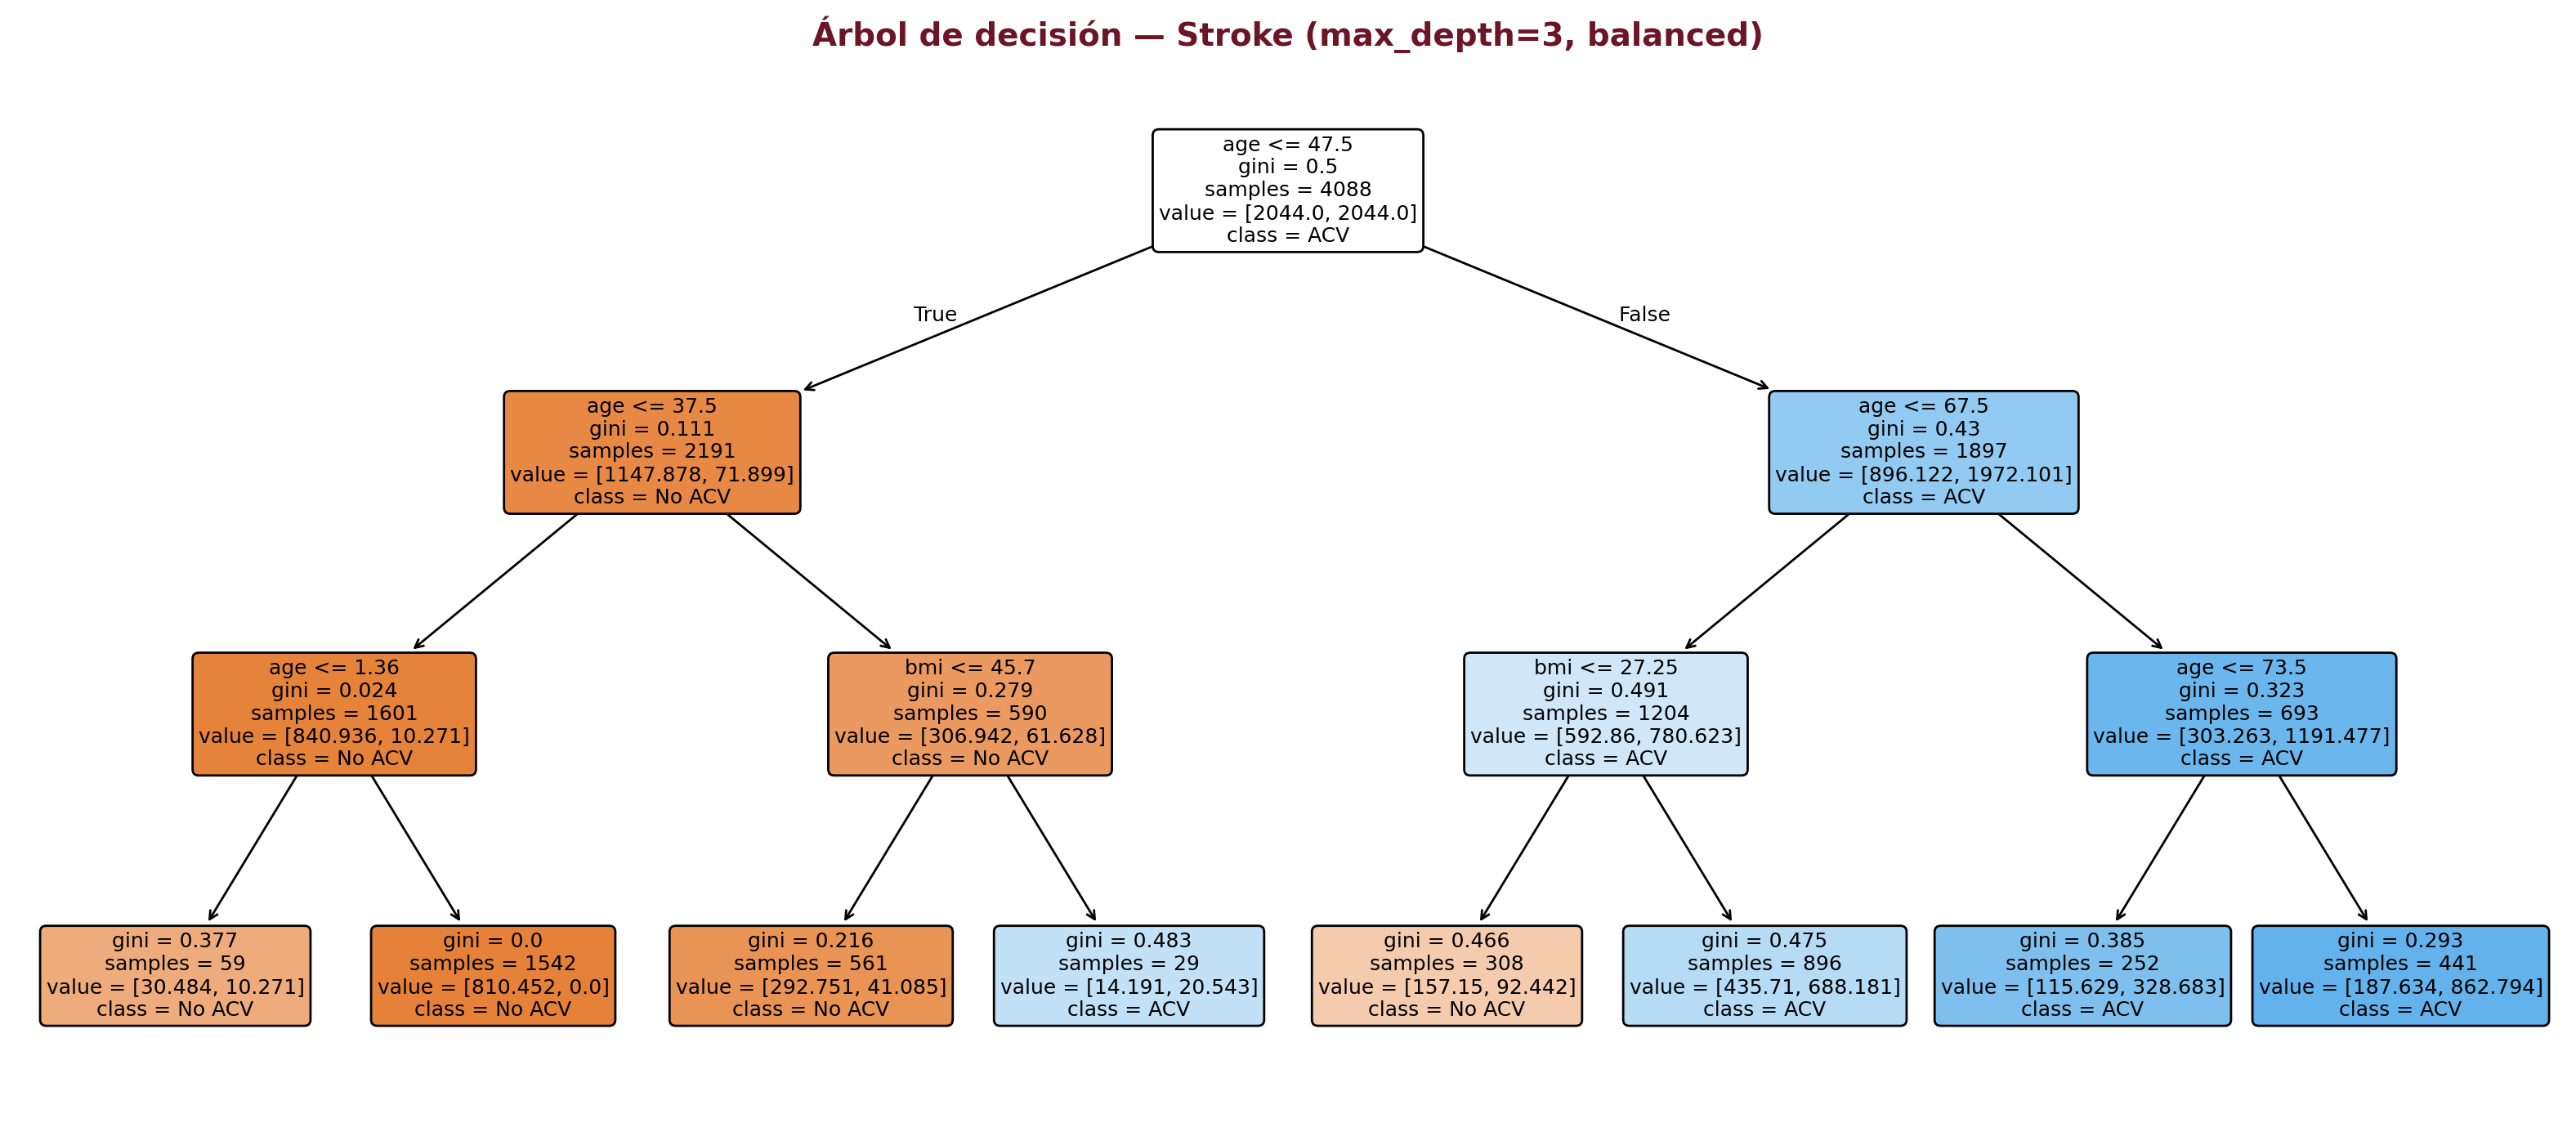
\includegraphics[width=0.95\textwidth]{fig_arbol_visual.png}
  \end{center}

  \vspace{-2pt}
  {\scriptsize\color{textMuted}
    \faLightbulb\hspace{4pt} \textbf{Cómo leerlo:}
    cada nodo dice la pregunta, el Gini, cuántas muestras caen ahí, y
    la distribución de clases. Sigue el camino para explicar cada predicción.}
\end{frame}

\begin{frame}[shrink=5]{Otros Hiperparámetros de Poda}
  \vspace{-4pt}
  {\footnotesize\color{arcaDark}\bfseries
    \texttt{max\_depth} es el más importante, pero hay más:}

  \vspace{6pt}
  {\scriptsize
  \begin{tabular}{@{}lp{6cm}p{3.5cm}@{}}
    \toprule
    \textbf{Parámetro} & \textbf{Qué hace} & \textbf{Valor sugerido} \\
    \midrule
    \texttt{max\_depth} & Máxima profundidad del árbol. & 3--8 para empezar. \\
    \texttt{min\_samples\_split} & Mín. muestras para hacer un corte. & 10--50. \\
    \texttt{min\_samples\_leaf} & Mín. muestras en cada hoja. & 5--20. \\
    \texttt{max\_features} & Cuántas variables evalúa por corte. & \texttt{None} (todas). \\
    \texttt{class\_weight} & Penalización por clase. & \texttt{"balanced"}. \\
    \bottomrule
  \end{tabular}
  }

  \vspace{6pt}
  {\scriptsize\color{textMuted}
    \faLightbulb\hspace{4pt} Empiecen con \texttt{max\_depth}.
    Si no es suficiente, agreguen \texttt{min\_samples\_leaf}.
    No ajusten todo a la vez.}
\end{frame}

\begin{frame}[shrink=5]{Ejercicio 2: Tu Primer Árbol}
  \vspace{-4pt}
  {\footnotesize\color{arcaDark}\bfseries
    \faClock\hspace{4pt} 10 minutos --- en el notebook:}

  \vspace{6pt}
  {\footnotesize
  \begin{enumerate}\setlength{\itemsep}{4pt}
    \item Entrenen un \texttt{DecisionTreeClassifier} sin límites.
    \item Reporten accuracy de train y test. ¿Hay overfitting?
    \item Ahora con \texttt{max\_depth=5} y \texttt{class\_weight="balanced"}.
    \item Visualicen el árbol con \texttt{plot\_tree}.
    \item Lean el camino desde la raíz: ¿cuál es la primera variable
      que pregunta? ¿Tiene sentido clínico?
  \end{enumerate}
  }
\end{frame}

% =============================================================================
%  BLOQUE G: OVERFITTING
% =============================================================================
\sectionframe{Overfitting}{El enemigo principal del árbol}

\begin{frame}{¿Qué Es Overfitting?}
  \vspace{-4pt}
  {\footnotesize\color{arcaDark}\bfseries
    Un modelo que \textbf{memoriza} los datos de entrenamiento en lugar
    de \textbf{aprender} patrones generalizables.}

  \vspace{8pt}
  \begin{columns}[T]
    \begin{column}{0.48\textwidth}
      \begin{tcolorbox}[colback=arcaRed!8, colframe=arcaRed, boxrule=0.5pt,
        arc=2pt, left=6pt, right=6pt, top=4pt, bottom=4pt,
        title={\small\color{white}\bfseries\faTimesCircle\ Overfitting}]
        {\scriptsize
        \begin{itemize}\setlength{\itemsep}{2pt}
          \item Train accuracy: 100\%
          \item Test accuracy: 90\%
          \item Brecha grande = memorización.
          \item No generaliza a datos nuevos.
        \end{itemize}
        }
      \end{tcolorbox}
    \end{column}
    \begin{column}{0.48\textwidth}
      \begin{tcolorbox}[colback=codeGreen!8, colframe=codeGreen, boxrule=0.5pt,
        arc=2pt, left=6pt, right=6pt, top=4pt, bottom=4pt,
        title={\small\color{white}\bfseries\faCheckCircle\ Buen ajuste}]
        {\scriptsize
        \begin{itemize}\setlength{\itemsep}{2pt}
          \item Train accuracy: 93\%
          \item Test accuracy: 91\%
          \item Brecha chica = generalización.
          \item Confiable en producción.
        \end{itemize}
        }
      \end{tcolorbox}
    \end{column}
  \end{columns}

  \vspace{6pt}
  {\scriptsize\color{textMuted}
    \faArrowRight\hspace{4pt} La logística rara vez hace overfitting (es simple).
    El árbol lo hace \textbf{siempre} si no lo podamos.}
\end{frame}

\begin{frame}[shrink=15]{Overfitting Visualizado: Train vs Test por Profundidad}
  \vspace{-4pt}
  \begin{center}
    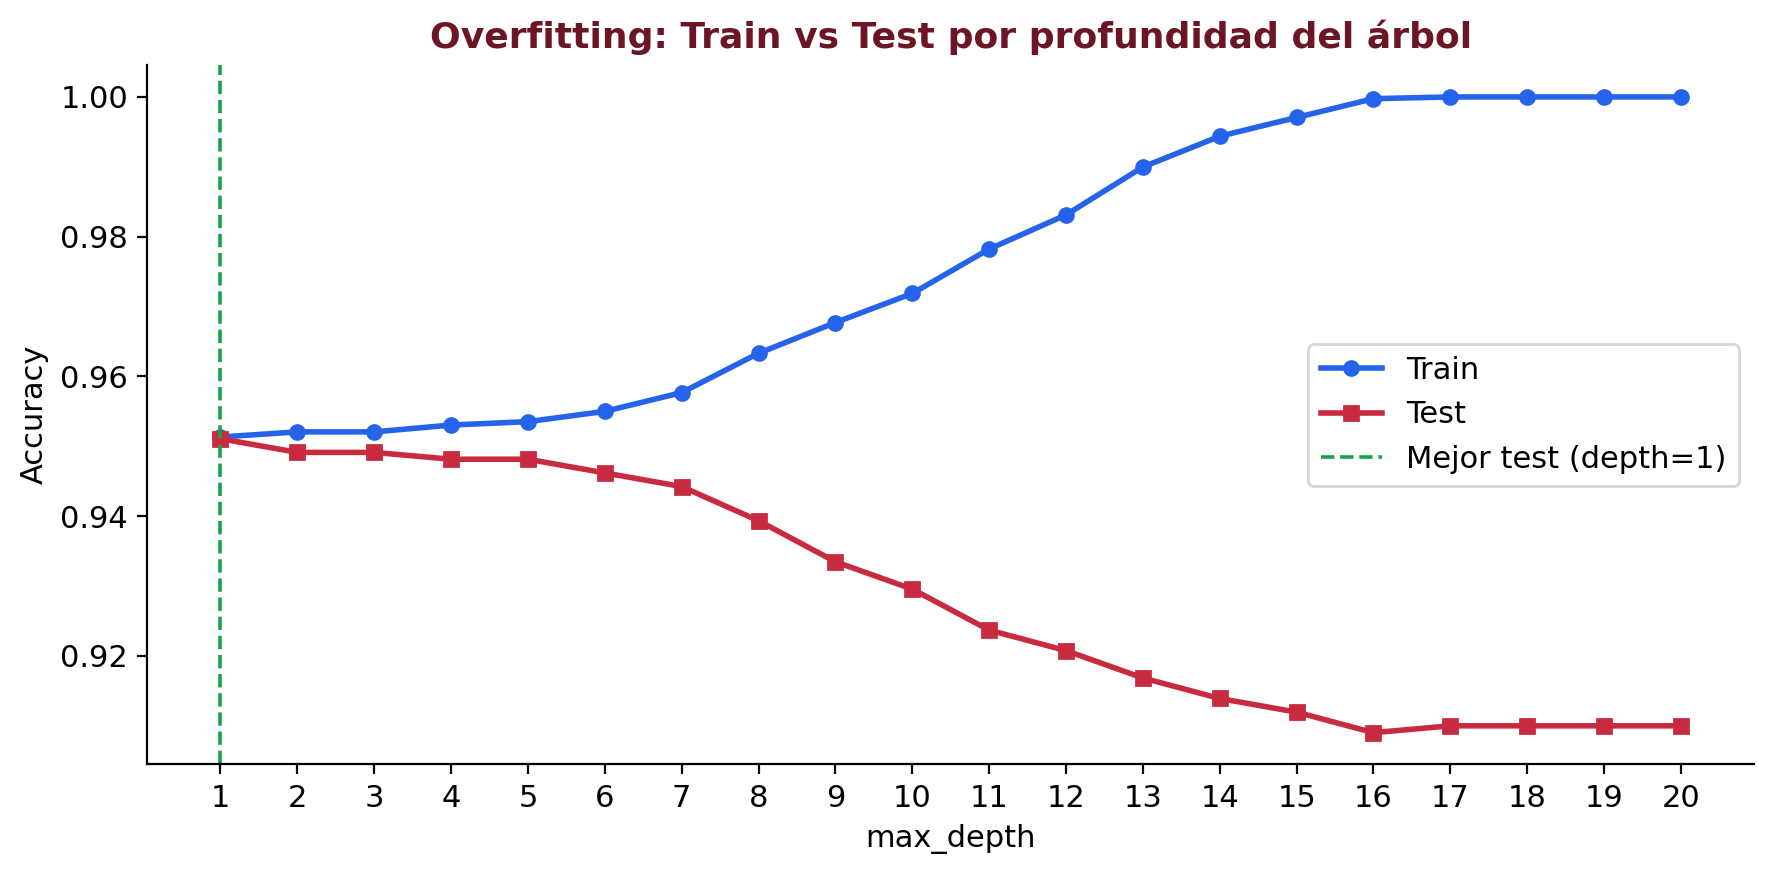
\includegraphics[width=0.8\textwidth]{fig_overfitting.png}
  \end{center}

  \vspace{-2pt}
  {\scriptsize\color{textMuted}
    \faLightbulb\hspace{4pt} \textbf{Clave:} el accuracy de train \textbf{siempre sube}
    al aumentar la profundidad. El de test \textbf{sube y luego baja}.
    El punto óptimo es donde el test es máximo.}
\end{frame}

\begin{frame}[fragile,shrink=22]{Código: Buscar el Mejor \texttt{max\_depth}}
  \vspace{-6pt}
  \begin{pyblock}
import numpy as np
resultados = []
for depth in range(1, 21):
    t = DecisionTreeClassifier(max_depth=depth,
            class_weight="balanced", random_state=42)
    t.fit(X_train, y_train)
    resultados.append({
        "depth": depth,
        "train": t.score(X_train, y_train),
        "test":  t.score(X_test, y_test)})

df_depth = pd.DataFrame(resultados)
mejor = df_depth.loc[df_depth["test"].idxmax()]
print(f"Mejor depth: {int(mejor['depth'])}")
print(f"  train: {mejor['train']:.3f}  test: {mejor['test']:.3f}")
  \end{pyblock}

  \vspace{4pt}
  {\scriptsize\color{arcaDark}
    \faKey\hspace{4pt} Elegir el \texttt{max\_depth} que maximiza el
    \textbf{test} --- no el train.}
\end{frame}

\begin{frame}[shrink=5]{Ejercicio 3: Busca tu Profundidad Óptima}
  \vspace{-4pt}
  {\footnotesize\color{arcaDark}\bfseries
    \faClock\hspace{4pt} 10 minutos --- en el notebook:}

  \vspace{6pt}
  {\footnotesize
  \begin{enumerate}\setlength{\itemsep}{4pt}
    \item Copia el código del barrido de profundidades (1 a 20).
    \item Graficá train vs test accuracy con Plotly (\texttt{px.line}).
    \item ¿Cuál es el mejor \texttt{max\_depth}?
    \item Entrená el árbol final con esa profundidad.
    \item \textbf{Bonus:} repite usando \texttt{recall\_score} en vez de
      accuracy. ¿Cambia el \texttt{max\_depth} óptimo?
  \end{enumerate}
  }
\end{frame}

% =============================================================================
%  BLOQUE H-pre: PROBABILIDADES Y DESBALANCE EN ÁRBOLES
% =============================================================================

\begin{frame}{¿El Árbol Devuelve Probabilidades? --- Sí}
  \vspace{-4pt}
  {\footnotesize\color{arcaDark}\bfseries
    Un paciente cae en una hoja. En esa hoja hay, digamos,
    30 pacientes de entrenamiento: 24 con ACV y 6 sanos.}

  \vspace{8pt}
  {\footnotesize
  \begin{itemize}\setlength{\itemsep}{5pt}
    \item[{\color{arcaRed}\scriptsize\faArrowRight}]
      \textbf{La clase predicha:} ACV (la mayoría).
    \item[{\color{arcaRed}\scriptsize\faArrowRight}]
      \textbf{La probabilidad:} $24/30 = 80\%$ de riesgo de ACV.
    \item[{\color{arcaRed}\scriptsize\faArrowRight}]
      Es simplemente la \textbf{proporción} de cada clase entre los
      pacientes de entrenamiento que cayeron en esa hoja.
  \end{itemize}
  }

  \vspace{6pt}
  \begin{tcolorbox}[colback=codeGreen!8, colframe=codeGreen, boxrule=0.5pt, arc=2pt,
    left=6pt, right=6pt, top=4pt, bottom=4pt]
    {\scriptsize\color{arcaDark}
    \faLightbulb\hspace{4pt}\textbf{Consecuencia:} como el árbol devuelve
    probabilidades, podemos hacer \textbf{todo} lo que hicimos con logística:
    curvas ROC, curvas PR, umbral óptimo.
    \texttt{arbol.predict\_proba()} funciona exactamente igual.}
  \end{tcolorbox}
\end{frame}

\begin{frame}[fragile,shrink=10]{Código: \texttt{predict\_proba} del Árbol}
  \vspace{-4pt}
  {\footnotesize\color{arcaDark}\bfseries
    La misma sintaxis que logística. Mismo patrón, distinto modelo.}

  \vspace{4pt}
  \begin{pyblock}
# Logistica
proba_lr = modelo.predict_proba(X_test_s)[:, 1]

# Arbol (nota: NO necesita datos escalados)
proba_arbol = arbol_podado.predict_proba(X_test)[:, 1]

# Ambos devuelven un array de probabilidades [0.0 ... 1.0]
# Ambos permiten calcular ROC, PR, umbral optimo
from sklearn.metrics import roc_auc_score
print(f"AUC logistica: {roc_auc_score(y_test, proba_lr):.3f}")
print(f"AUC arbol:     {roc_auc_score(y_test, proba_arbol):.3f}")
  \end{pyblock}

  \vspace{4pt}
  {\scriptsize\color{textMuted}
    \faKey\hspace{4pt} El patrón \texttt{modelo.predict\_proba()[:, 1]}
    es \textbf{universal} en sklearn. Funciona con logística, árboles,
    random forest, SVM\ldots Siempre devuelve probabilidades.}
\end{frame}

\begin{frame}{Desbalance en Árboles: \texttt{class\_weight="balanced"}}
  \vspace{-4pt}
  {\footnotesize\color{arcaDark}\bfseries
    El mismo problema de clase 15: si el 95\% de los pacientes son sanos,
    el árbol puede ignorar los enfermos y tener accuracy ``alta''.}

  \vspace{6pt}
  {\footnotesize
  \begin{itemize}\setlength{\itemsep}{5pt}
    \item[{\color{arcaRed}\scriptsize\faTimesCircle}]
      \textbf{Sin balancear:} el árbol optimiza accuracy → predice
      ``sano'' casi siempre → recall bajo.
    \item[{\color{codeGreen}\scriptsize\faCheckCircle}]
      \textbf{Con \texttt{class\_weight="balanced"}:} le dice al árbol que
      un error en la clase minoritaria (ACV) \textbf{pesa más} que un error
      en la mayoría (sano). El árbol se esfuerza más en detectar ACV.
    \item[{\color{codeGreen}\scriptsize\faCheckCircle}]
      Es la \textbf{misma técnica} que usamos en logística (clase 15).
      Funciona igual.
  \end{itemize}
  }

  \vspace{6pt}
  \begin{tcolorbox}[colback=arcaGray, colframe=arcaRed, boxrule=0.5pt, arc=2pt,
    left=6pt, right=6pt, top=4pt, bottom=4pt]
    {\scriptsize\color{arcaDark}
    \faExclamationTriangle\hspace{4pt}\textbf{Regla:} si los datos están
    desbalanceados, \textbf{siempre} usen \texttt{class\_weight="balanced"}
    tanto en logística como en árboles. Es una sola línea de código.}
  \end{tcolorbox}
\end{frame}

% =============================================================================
%  BLOQUE H: FEATURE IMPORTANCE + COMPARACIÓN
% =============================================================================
\sectionframe{Feature Importance}{Qué variables mandan}

\begin{frame}{¿Cómo Mide la Importancia el Árbol?}
  \vspace{-4pt}
  {\footnotesize\color{arcaDark}\bfseries
    Cada vez que el árbol usa una variable para hacer un corte,
    reduce la impureza. La \textbf{importancia} de una variable es
    cuánto reduce la impureza \textit{en total}.}

  \vspace{6pt}
  {\footnotesize
  \begin{itemize}\setlength{\itemsep}{5pt}
    \item[{\color{arcaRed}\scriptsize\faArrowRight}]
      Si ``edad'' aparece en 5 nodos y cada vez reduce mucho el Gini
      → importancia alta.
    \item[{\color{arcaRed}\scriptsize\faArrowRight}]
      Si ``gender\_Male'' solo aparece en 1 nodo y reduce poco
      → importancia baja.
    \item[{\color{arcaRed}\scriptsize\faArrowRight}]
      Las importancias suman 1.0 (normalizadas).
  \end{itemize}
  }

  \vspace{6pt}
  \begin{tcolorbox}[colback=arcaGray, colframe=arcaRed, boxrule=0.5pt, arc=2pt,
    left=6pt, right=6pt, top=4pt, bottom=4pt]
    {\scriptsize\color{arcaDark}
    \faLightbulb\hspace{4pt}\textbf{Ventaja sobre logística:} no necesita
    escalado. Funciona con variables en escalas distintas.
    No asume relación lineal.}
  \end{tcolorbox}
\end{frame}

\begin{frame}[fragile,shrink=18]{Código: \texttt{feature\_importances\_}}
  \vspace{-6pt}
  \begin{pyblock}
import pandas as pd
import plotly.express as px

importancias = pd.DataFrame({
    "feature": X_train.columns,
    "importancia": arbol_podado.feature_importances_
}).sort_values("importancia", ascending=True).tail(10)

fig = px.bar(importancias, x="importancia", y="feature",
             orientation="h",
             title="Top 10 variables mas importantes (arbol)")
fig.show()
  \end{pyblock}

  \vspace{4pt}
  {\scriptsize\color{textMuted}
    \faArrowRight\hspace{4pt} \texttt{feature\_importances\_}: array con la
    importancia de cada variable. Se accede después de \texttt{.fit()}.}
\end{frame}

\begin{frame}[shrink=15]{Importancia: Árbol vs Logística}
  \vspace{-4pt}
  \begin{center}
    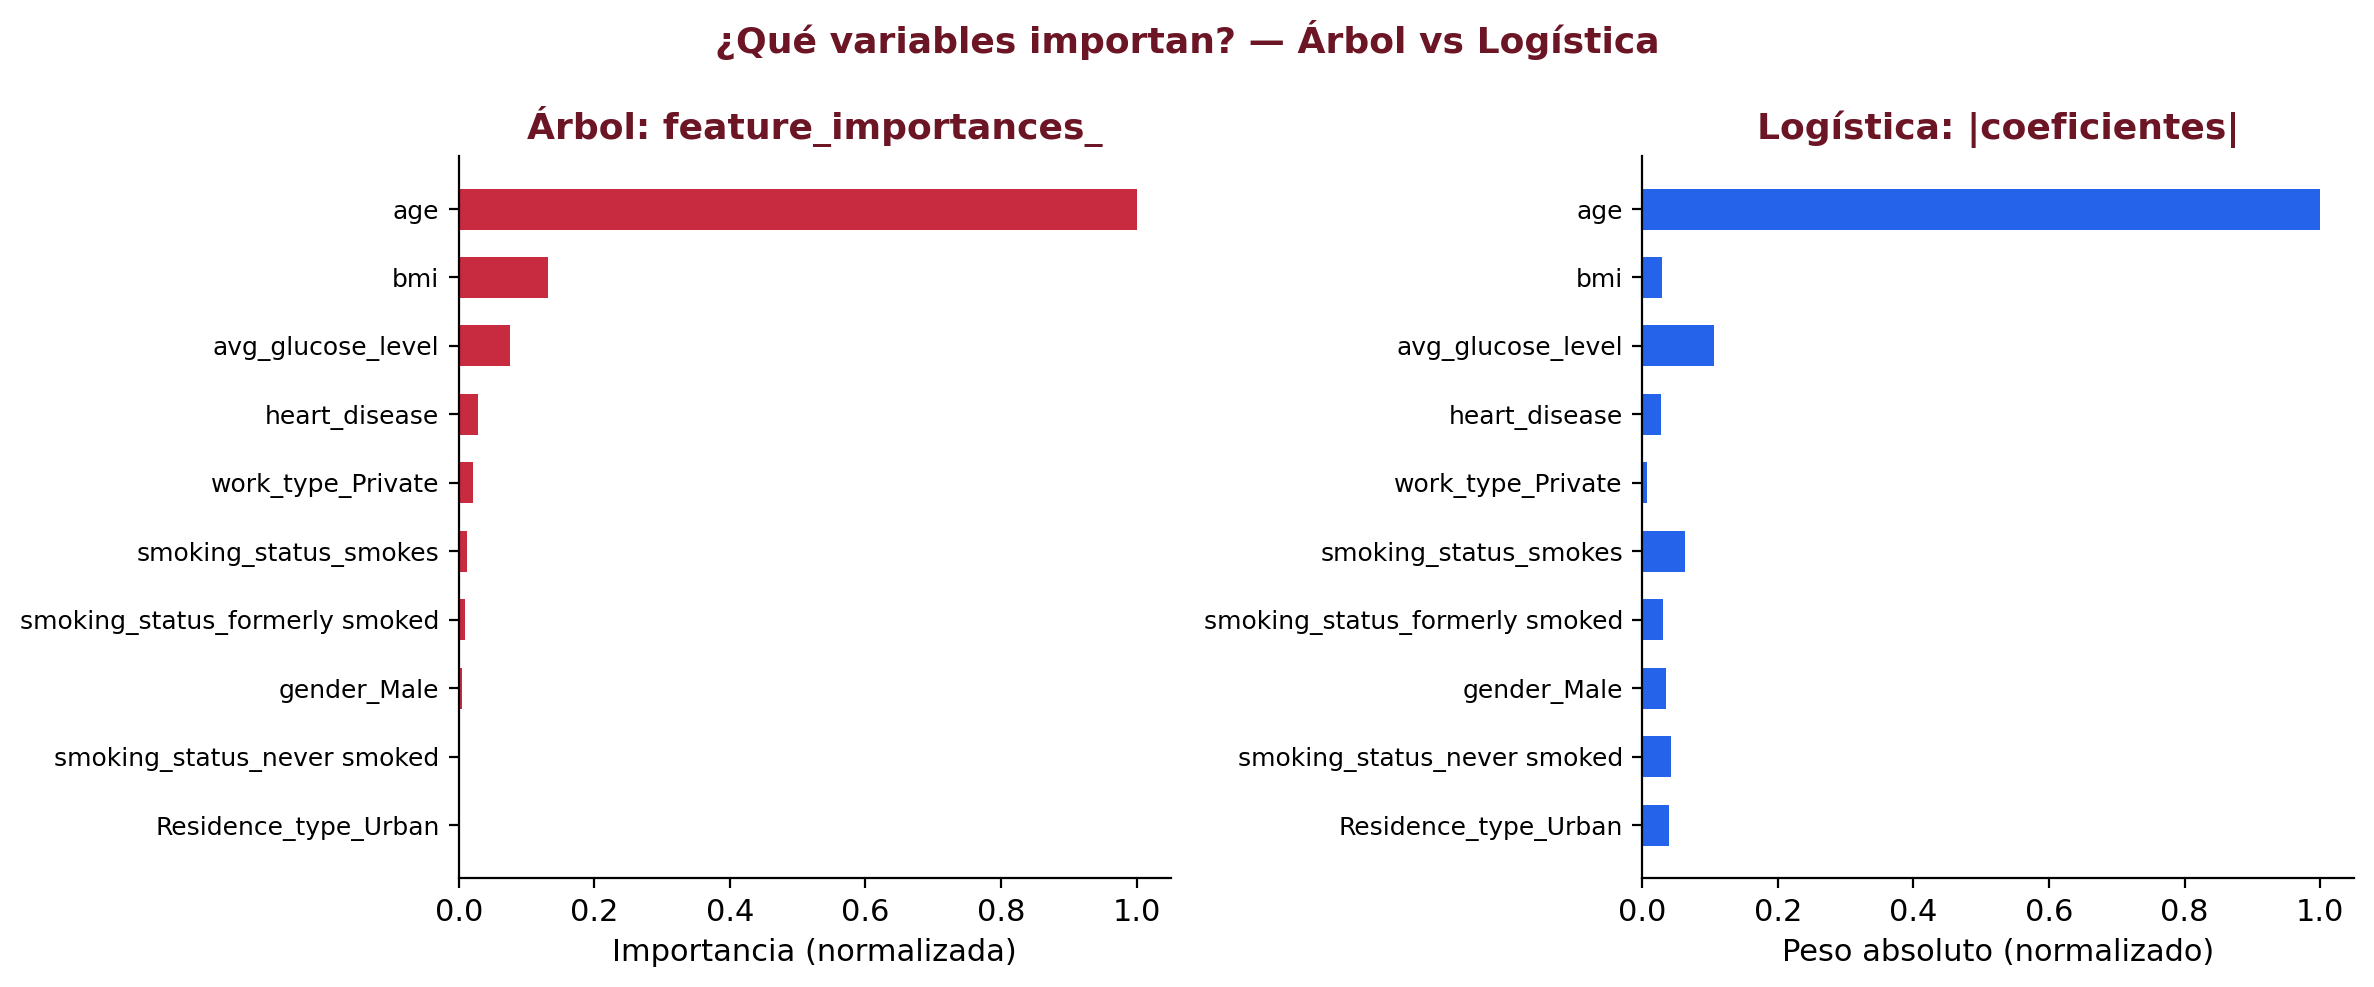
\includegraphics[width=0.88\textwidth]{fig_importances.png}
  \end{center}

  \vspace{-2pt}
  {\scriptsize\color{textMuted}
    \faLightbulb\hspace{4pt} Las dos coinciden en que \textbf{edad} es la
    variable más importante. Pero difieren en las siguientes.
    Eso es normal: miden importancia de formas distintas
    (reducción de Gini vs peso en la ecuación lineal).}
\end{frame}

\begin{frame}[fragile,shrink=25]{Comparar en las Mismas Métricas}
  \vspace{-6pt}
  \begin{pyblock}
from sklearn.metrics import (classification_report,
                             roc_auc_score)

# Arbol
y_pred_arbol = arbol_podado.predict(X_test)
y_prob_arbol = arbol_podado.predict_proba(X_test)[:, 1]

# Logistica (ya entrenada con X_test_s)
y_pred_lr = modelo.predict(X_test_s)
y_prob_lr = modelo.predict_proba(X_test_s)[:, 1]

print("=== ARBOL ===")
print(classification_report(y_test, y_pred_arbol,
                            target_names=["No ACV","ACV"]))
print(f"AUC: {roc_auc_score(y_test, y_prob_arbol):.3f}")
print("\n=== LOGISTICA ===")
print(classification_report(y_test, y_pred_lr,
                            target_names=["No ACV","ACV"]))
print(f"AUC: {roc_auc_score(y_test, y_prob_lr):.3f}")
  \end{pyblock}
\end{frame}

\begin{frame}[fragile,shrink=18]{Ambas Curvas ROC en un Solo Gráfico}
  \vspace{-6pt}
  \begin{pyblock}
import plotly.graph_objects as go

fpr_lr, tpr_lr, _ = roc_curve(y_test, y_prob_lr)
fpr_t, tpr_t, _ = roc_curve(y_test, y_prob_arbol)

fig = go.Figure()
fig.add_trace(go.Scatter(x=fpr_lr, y=tpr_lr, mode="lines",
    name=f"Logistica (AUC={roc_auc_score(y_test,y_prob_lr):.3f})"))
fig.add_trace(go.Scatter(x=fpr_t, y=tpr_t, mode="lines",
    name=f"Arbol (AUC={roc_auc_score(y_test,y_prob_arbol):.3f})"))
fig.add_shape(type="line", line=dict(dash="dash"),
              x0=0,x1=1,y0=0,y1=1)
fig.update_layout(title="ROC: Logistica vs Arbol",
    xaxis_title="FPR", yaxis_title="TPR")
fig.show()
  \end{pyblock}
\end{frame}

\begin{frame}[shrink=5]{Resumen: Cuándo Usar Cada Modelo}
  \vspace{-4pt}
  {\scriptsize
  \begin{tabular}{@{}p{3.5cm}p{4.5cm}p{4.5cm}@{}}
    \toprule
     & \textbf{\color{codeBlue}Logística} & \textbf{\color{arcaRed}Árbol} \\
    \midrule
    \textbf{Interpretación} & Coeficientes (peso de cada variable). & Caminos legibles. \\
    \textbf{Preprocesamiento} & Necesita escalado y encoding. & No necesita escalado. \\
    \textbf{Relación con target} & Asume relación lineal. & Captura no linealidad. \\
    \textbf{Overfitting} & Raro (modelo simple). & Frecuente (podar siempre). \\
    \textbf{Mejor para\ldots} & Relaciones lineales, pocos datos, regulaciones estrictas. & Interacciones complejas, explicar a no técnicos, base para ensambles. \\
    \bottomrule
  \end{tabular}
  }

  \vspace{6pt}
  \begin{tcolorbox}[colback=arcaGray, colframe=arcaRed, boxrule=0.5pt, arc=2pt,
    left=6pt, right=6pt, top=4pt, bottom=4pt]
    {\scriptsize\color{arcaDark}
    \faKey\hspace{4pt}\textbf{No hay modelo universal.} En la vida real,
    entrenamos ambos y elegimos con métricas.
    Próxima clase: ¿qué pasa si entrenamos \textbf{100 árboles a la vez}?}
  \end{tcolorbox}
\end{frame}

\begin{frame}[shrink=5]{Ejercicio 4: Comparación Completa}
  \vspace{-4pt}
  {\footnotesize\color{arcaDark}\bfseries
    \faClock\hspace{4pt} 12 minutos --- en el notebook:}

  \vspace{6pt}
  {\footnotesize
  \begin{enumerate}\setlength{\itemsep}{4pt}
    \item Entrenen logística y árbol (con mejor \texttt{max\_depth}).
    \item Para ambos: precision, recall, f1, AUC, AP.
    \item Grafiquen ambas curvas ROC en un solo gráfico.
    \item Grafiquen ambas curvas PR en un solo gráfico.
    \item ¿Cuál modelo elegirían para el hospital y por qué?
    \item \textbf{Bonus:} traduzcan el árbol a reglas de negocio usando
      \texttt{export\_text} de sklearn.
  \end{enumerate}
  }
\end{frame}

% =============================================================================
%  BLOQUE I: GRADIO — DEL NOTEBOOK A LA DEMO
% =============================================================================
\sectionframe{Gradio}{Del notebook a la demo interactiva}

\begin{frame}{El Último Paso: Entregar el Modelo}
  \vspace{-4pt}
  {\footnotesize\color{arcaDark}\bfseries
    Ya saben entrenar, evaluar y comparar modelos.
    Pero un notebook no se le entrega a un médico ni a un gerente.}

  \vspace{8pt}
  {\footnotesize
  \begin{itemize}\setlength{\itemsep}{5pt}
    \item[{\color{arcaRed}\scriptsize\faArrowRight}]
      En la vida real, el modelo vive dentro de una \textbf{aplicación}.
    \item[{\color{arcaRed}\scriptsize\faArrowRight}]
      La mayoría de APIs de predicción funcionan igual:
      \textbf{input → modelo.predict() → output}.
    \item[{\color{arcaRed}\scriptsize\faArrowRight}]
      \textbf{Gradio} permite crear esa interfaz en \textbf{5 líneas}.
      Funciona dentro de Jupyter.
  \end{itemize}
  }

  \vspace{6pt}
  \begin{tcolorbox}[colback=codePurple!8, colframe=codePurple, boxrule=0.5pt, arc=2pt,
    left=6pt, right=6pt, top=4pt, bottom=4pt]
    {\scriptsize\color{arcaDark}
    \faLightbulb\hspace{4pt}\textbf{Patrón universal:} ya sea Flask, FastAPI,
    Streamlit, Dash o Gradio --- todos siguen la misma idea.
    Input del usuario → función → output. Gradio es el más simple de todos.}
  \end{tcolorbox}
\end{frame}

\begin{frame}{¿Qué Es Gradio?}
  \vspace{-4pt}
  {\footnotesize\color{arcaDark}\bfseries
    Una librería Python que crea interfaces web \textbf{interactivas}
    para funciones de ML. Ideal para demos.}

  \vspace{6pt}
  {\scriptsize
  \begin{tabular}{@{}lp{5cm}p{5cm}@{}}
    \toprule
    \textbf{Herramienta} & \textbf{Para qué} & \textbf{Complejidad} \\
    \midrule
    \textbf{\color{codePurple}Gradio} & Demos rápidas de modelos ML. & 5--10 líneas. \\
    \textbf{Streamlit} & Dashboards y apps de datos. & 20--50 líneas. \\
    \textbf{Dash (Plotly)} & Dashboards interactivos complejos. & 50+ líneas. \\
    \textbf{Flask / FastAPI} & APIs REST completas. & 100+ líneas. \\
    \bottomrule
  \end{tabular}
  }

  \vspace{6pt}
  {\scriptsize\color{textMuted}
    \faArrowRight\hspace{4pt} Hoy usamos Gradio porque queremos ir
    del modelo a la demo en \textbf{minutos}, no horas.
    Las otras herramientas las verán cuando necesiten algo más complejo.}
\end{frame}

\begin{frame}[fragile,shrink=22]{Tu Primera Demo: Predictor de ACV}
  \vspace{-6pt}
  \begin{pyblock}
import gradio as gr

def predecir_acv(edad, glucosa_promedio, bmi,
                 hipertension, enfermedad_cardiaca):
    # Crear el vector de entrada con el mismo formato del train
    datos = pd.DataFrame([{
        "age": edad,
        "avg_glucose_level": glucosa_promedio,
        "bmi": bmi,
        "hypertension": int(hipertension),
        "heart_disease": int(enfermedad_cardiaca),
        # ... resto de features con valores por defecto
    }])
    datos_enc = # encoding igual que en train
    proba = arbol_podado.predict_proba(datos_enc)[0, 1]
    return f"Riesgo de ACV: {proba:.1%}"

demo = gr.Interface(
    fn=predecir_acv,
    inputs=[
        gr.Slider(0, 100, value=50, label="Edad"),
        gr.Slider(50, 300, value=100, label="Glucosa promedio"),
        gr.Slider(10, 50, value=25, label="BMI"),
        gr.Checkbox(label="Hipertension"),
        gr.Checkbox(label="Enfermedad cardiaca"),
    ],
    outputs="text",
    title="Predictor de Riesgo de ACV")
demo.launch()
  \end{pyblock}
\end{frame}

\begin{frame}{Anatomía de \texttt{gr.Interface}}
  \vspace{-4pt}
  {\footnotesize\color{arcaDark}\bfseries
    Tres piezas. Es todo lo que necesitan:}

  \vspace{6pt}
  {\footnotesize
  \begin{enumerate}\setlength{\itemsep}{6pt}
    \item[{\color{arcaRed}\bfseries fn}]
      Tu \textbf{función Python}. Recibe los inputs, retorna el output.
      Dentro llama a \texttt{modelo.predict\_proba()}.
    \item[{\color{arcaRed}\bfseries inputs}]
      Lista de \textbf{componentes de entrada}: sliders, checkboxes,
      dropdowns, text boxes.
    \item[{\color{arcaRed}\bfseries outputs}]
      El tipo de \textbf{salida}: texto, número, gráfico, tabla.
  \end{enumerate}
  }

  \vspace{6pt}
  {\scriptsize
  \begin{tabular}{@{}llp{6cm}@{}}
    \toprule
    \textbf{Componente} & \textbf{Gradio} & \textbf{Cuándo usarlo} \\
    \midrule
    Slider & \texttt{gr.Slider(0, 100)} & Variables continuas (edad, glucosa). \\
    Checkbox & \texttt{gr.Checkbox()} & Variables binarias (sí/no). \\
    Dropdown & \texttt{gr.Dropdown([...~])} & Variables categóricas (género, trabajo). \\
    Number & \texttt{gr.Number()} & Cualquier número libre. \\
    \bottomrule
  \end{tabular}
  }
\end{frame}

\begin{frame}[fragile,shrink=10]{Compartir tu Demo}
  \vspace{-4pt}
  {\footnotesize\color{arcaDark}\bfseries
    Con \texttt{share=True}, Gradio genera un \textbf{link público}
    temporal (72 horas). Cualquiera puede usarlo.}

  \vspace{6pt}
  \begin{pyblock}
demo.launch(share=True)
# -> Running on public URL: https://xxxxx.gradio.live
  \end{pyblock}

  \vspace{6pt}
  {\footnotesize
  \begin{itemize}\setlength{\itemsep}{5pt}
    \item[{\color{codeGreen}\scriptsize\faCheckCircle}]
      El médico abre el link en su celular y prueba pacientes.
    \item[{\color{codeGreen}\scriptsize\faCheckCircle}]
      El gerente ve que el modelo ``funciona de verdad''.
    \item[{\color{codeGreen}\scriptsize\faCheckCircle}]
      No necesitas servidor, hosting ni deployment.
    \item[{\color{arcaRed}\scriptsize\faTimesCircle}]
      El link expira en 72h. Para producción real,
      se usan Hugging Face Spaces o APIs con FastAPI.
  \end{itemize}
  }
\end{frame}

\begin{frame}[shrink=5]{Ejercicio 5: Tu Demo con Gradio}
  \vspace{-4pt}
  {\footnotesize\color{arcaDark}\bfseries
    \faClock\hspace{4pt} 12 minutos --- en el notebook:}

  \vspace{6pt}
  {\footnotesize
  \begin{enumerate}\setlength{\itemsep}{4pt}
    \item Instalar: \texttt{!pip install gradio}
    \item Completen la función \texttt{predecir\_acv} con el modelo entrenado.
    \item Lancen la demo con \texttt{demo.launch()}.
    \item Prueben con un paciente de 70 años, glucosa 220, hipertenso.
    \item Prueben con uno de 25 años, glucosa 80, sano.
    \item ¿Los resultados tienen sentido clínico?
    \item \textbf{Bonus:} agreguen un \texttt{gr.Dropdown} para
      ``tipo de trabajo'' o ``estado de tabaquismo''.
  \end{enumerate}
  }
\end{frame}

% =============================================================================
%  CIERRE
% =============================================================================
\sectionframe{Cierre}{Lo que aprendimos hoy}

\begin{frame}[shrink=8]{Resumen}
  \vspace{-4pt}
  \begin{columns}[T]
    \begin{column}{0.48\textwidth}
      {\footnotesize\bfseries\color{arcaDark} Evaluación:}
      \vspace{4pt}

      {\footnotesize
      \begin{itemize}\setlength{\itemsep}{4pt}
        \item[{\color{codeGreen}\faCheckCircle}]
          Curva ROC + AUC.
        \item[{\color{codeGreen}\faCheckCircle}]
          Curva PR + AP (para desbalanceados).
        \item[{\color{codeGreen}\faCheckCircle}]
          Umbral óptimo por costo de negocio.
      \end{itemize}
      }

      \vspace{6pt}
      {\footnotesize\bfseries\color{arcaDark} Deployment:}
      \vspace{4pt}

      {\footnotesize
      \begin{itemize}\setlength{\itemsep}{4pt}
        \item[{\color{codeGreen}\faCheckCircle}]
          Gradio: del notebook a la demo en 5 líneas.
        \item[{\color{codeGreen}\faCheckCircle}]
          Patrón input → predict → output.
      \end{itemize}
      }
    \end{column}

    \begin{column}{0.48\textwidth}
      {\footnotesize\bfseries\color{arcaRed} Árboles de decisión:}
      \vspace{4pt}

      {\footnotesize
      \begin{itemize}\setlength{\itemsep}{4pt}
        \item[{\color{codeGreen}\faCheckCircle}]
          Diagrama de flujo interpretable.
        \item[{\color{codeGreen}\faCheckCircle}]
          Gini mide impureza, elige los cortes.
        \item[{\color{codeGreen}\faCheckCircle}]
          Overfitting → podar con \texttt{max\_depth}.
        \item[{\color{codeGreen}\faCheckCircle}]
          \texttt{feature\_importances\_} para saber qué pesa.
      \end{itemize}
      }
    \end{column}
  \end{columns}

  \vspace{8pt}
  \begin{tcolorbox}[colback=arcaRed!8, colframe=arcaRed, boxrule=0.5pt, arc=2pt,
    left=6pt, right=6pt, top=4pt, bottom=4pt]
    {\scriptsize\color{arcaDark}
    \faArrowRight\hspace{4pt}\textbf{Próxima clase:} Random Forest
    --- ``¿qué pasa si entrenamos 100 árboles y los hacemos votar?''
    Spoiler: funciona \textit{muy} bien.}
  \end{tcolorbox}
\end{frame}

% ── QR ENCUESTA ──────────────────────────────────────────────────────────────
{
\setbeamertemplate{headline}{}
\setbeamertemplate{footline}{}
\begin{frame}[plain, noframenumbering]
  \begin{tikzpicture}[remember picture, overlay]
    \fill[arcaDark] (current page.south west) rectangle (current page.north east);
  \end{tikzpicture}
  \vspace{1cm}
  \begin{center}
    {\Huge\bfseries\color{white} ¿Cómo estuvo la clase?\par}
    \vspace{0.6cm}
    
\includegraphics[width=4cm]{qr_encuesta.jpg}
    \vspace{0.4cm}

    {\large\color{white!80} Escanea el QR para dejarnos tu opinión.\par}
  \end{center}
\end{frame}
}

\end{document}
